%
% Template for Doctoral Theses at Uppsala 
% University. The template is based on    
% the layout and typography used for      
% dissertations in the Acta Universitatis 
% Upsaliensis series                      
% Ver 5.2 - 2012-08-08                  
% Latest version available at:            
%   http://ub.uu.se/thesistemplate            
%                                         
% Support: Wolmar Nyberg Akerstrom        
% Thesis Production           
% Uppsala University Library              
% avhandling@ub.uu.se                          
%                                         
%%%%%%%%%%%%%%%%%%%%%%%%%%%%%%%%%%%%%%%%%%%


\documentclass[10pt, a4paper]{UUThesisTemplate}

% Package to determine wether XeTeX is used

	% XeTeX specific packages and settings
	% Language, diacritics and hyphenation
\usepackage[babelshorthands]{polyglossia}
\setmainlanguage{english}
\setotherlanguages{swedish}


	% Font settings
\setmainfont{Hoefler Text}
\setromanfont{Hoefler Text}
\setsansfont{Verdana}[Scale=MatchLowercase]
\setmonofont{Consolas}[Scale=MatchLowercase]
\newfontfamily{\C}{STXihei}[Scale=MatchUppercase]

\usepackage{graphicx}
% Tables
\usepackage{booktabs}
\usepackage{microtype}
\usepackage{tabularx}
\usepackage{amsmath}
\usepackage{amssymb}
\usepackage{wrapfig}
\usepackage{tikz}
\usetikzlibrary{datavisualization}
\usetikzlibrary{backgrounds}
\usepackage{listings}
\usepackage{marginnote}
\usepackage{pdfpages}
\usepackage{lineno}
\usepackage{multirow}
%\linenumbers

\input{listing_definitions.tex}

\pgfdeclaredataformat{commentcountdata}%
    {}{}{#1, #2, #3}
    {%
    \pgfkeys{/data point/.cd,count=#1, y=#2, set=sportsmole} \pgfdatapoint
    \pgfkeys{/data point/.cd,count=#1, y=#3, set=goal} \pgfdatapoint
    }{}{}%



\definecolor{goal_blue}{RGB}{0, 100, 163}
\definecolor{sportsmole_green}{RGB}{69, 125, 20}

\pgfdvdeclarestylesheet{football commentary}{
  1/.style={black},
  2/.style={black},
  3/.style={black},
}

% Document links and bookmarks
\usepackage{hyperref} 

% Numbering of headings down to the subsection level
\numberingdepth{section}

% Including headings down to the subsection level in contents
\contentsdepth{chapter}


\author{Maximilian Balthasar Mansky}
\titlepagelogo{\includegraphics{UU_logo_sv_42.eps}}
\title{Mapping from physical events to words using neural networks}
\subtitle{A case study on football}



% Uncomment to use a custom abstract dummy text
\abstractdummy{
\begin{center}%
\begin{minipage}{8cm}
\vspace{10cm}
\begin{abstract}
A neural network around a football game is examined, with the feature data being ball positions and the label data human written commentary. The ball positions are successfully classified and text can be generated via LSTM networks similar to the human commentary. The final link between ball positions and commentary could not be made, due to too large of a difference in information content.
\end{abstract}
\end{minipage}
\end{center}
}


\begin{document}
\frontmatter
    % Creates the front matter (title page(s), abstract, list of papers)
    % for either a Comprehensive Summary or a Monograph.
    % Authors of Comprehensive Summaries use this front matter 
    \frontmatterCS 
    % Monograph authors use this front matter 
    %\frontmatterMonograph 
 
   % Optional dedication
   \dedication{\includegraphics[width=10cm]{figures/tchaikovsky_bassoon.png}\\Tchaikovsky 4th symphony, 2nd mvt, Andantino. Bassoon Solo}
    \begingroup
        % To adjust the indentation in your table of contents, uncomment and enter the widest numbers for each level
        %  E.g.  \settocnumwidth{widest chapter number}{widest section number}{widest subsection number}...{...}
       %  \settocnumwidth{5}{4}{5}{3}{3}{3}
       \setcounter{secnumdepth}{1}
        \tableofcontents
    \endgroup
    
    % Optional tables
    %\listoftables
    %\listoffigures

\mainmatter

\chapter{Introduction}

Physics is an understanding of the link between two different sets of physical realities, in particular microscopic actions and macroscopic effects. The latter describes what is measured in a laboratory; the aggregate effect of many small, microscopic interactions that together define what happens on the large scale.

Consider the example of a material; The microscopic constituents, the individual atoms and the relations to their nearest neighbours define the macroscopic behaviour such as conductivity, malleability, hardness and other quantifiable properties \cite{materialsc}. Both the choice of atoms and their arrangement lead to the intricate, complex and sometimes surprising behaviour seen on a larger scale [ibid.]. In a semiconductor, the base material of silicon changes its properties based on different atoms injected in the crystal (doping) \cite{feynman}. The resulting doped semiconductors have different properties. This classification relates to a third level of understanding that is much broader – The understanding of how nature and mathematics relate and the explanation thereof through the use of natural languages.

These three layers of understanding – the microscopic effects of the silicon atoms in the semiconductor and their interaction with the doping atoms, the macroscopic effects measured, such as resistivity, voltage drop, gate current and others and the explanation that links the two through explanation – form a tripartite view of reality. All three are necessary to use newly a newly grown understanding. To return to the case of the semiconductor, the knowledge of with which atoms to dope the material allows changing the macroscopic properties and create the transistors that power our modern experience of the world. Language also helps understanding the macroscopic effects through classification. In the simplest case, a semiconductor can be classified as an $p$- or $n$ type, depending on whether the doping introduces more ($n$-type) or less ($p$-type) electrons to the semiconductor base \cite{feynman}. The classification is a kind of alphabet that allows a description of the semiconductor. In this case it is a rather simple one with just two words, $n$-type or $p$-type. So for each microscopic action and arrangement, there is a macroscopic effect and classification thereof.

The requirement of classifying and grouping similar observed behaviour is also apparent in other fields of physics, in particular it is a feature in the field of complex systems, where a direct link between microscopic action and macroscopic behaviour cannot always be found. The physics of complex systems tries to describe the aggregate behaviour of complex interactions – often the behaviour of independent entities. Parts of the actions of the microscopic entities can be simulated in order to understand their part in the observed macroscopic effects \cite{flocking}. An example here is the flocking behaviour of some kinds of animals, in particular schools of fish or starling swarms [ibid.]. In a sense, these simulations approximate the analytical link between microscopic and macroscopic action. There are too many variables in a single entity, be it a bird or fish, so there is a reduction the most obvious ones that taken into account in the simulation.

Simulations as a means of finding mathematical links are also pat of this thesis. Parallel to the rise in computing power, the idea of self-learning machines has taken shape \cite{NN}. In the form of neural networks, machines have become successful at identifying correlations in data and classifying aspects of reality [ibid.]. Their power lies in finding regularities in vast quantities of data and classifying the data along clear lines. In a sense, neural networks allow to approximate the mathematical links through the correlations that arise from the casual connections. By classification, neural networks can link from microscopic data to the language description of the physical system, through an approximation of the macroscopic effects in the internal states of the network.

\section{Football as a physical system}

A football match can be understood as a physical system in the sense of the above. It can be classified as a complex system, based around the interactions of the 22 participating football players. While there is a clear link between some properties of the game and its final score (i.e. how often the ball has landed in the goal), the intermediary actions are much harder to grasp in an analytical way. The distribution of players can potentially be modeled as a thin gas, with the ball as an attractor. This is based on the observation that players spread over the field and cluster around the ball. The way that the ball is passed however, is more reminiscent of a complex system, principally dependent of the players decision that in turn depend on the actions of the players around, the current game situation and the position on the field.

In the context of this thesis, the core aspect of the physical system are two different descriptions of a match. Firstly, the ball position over time, as possession over it changes, players interact with it and it ultimately decides the score of the game. On the other hand is a description of the game through words – written commentary describing the current match. These two descriptions ostensibly describe the same physical situation, but are very different in their information. Because they are so different, there is little hope in finding a clear analytical relationship in the sense of hard physics, but instead it may be possible to find correlations that indicate a relationship, more along the lines of complex systems.

The macroscopic elements that describe a football match are laid out in the rules of the game. They are laid out in authoritative detail in \cite{footballrules}.  In the course of this thesis, the following subset of the rules is used:

\begin{itemize}
\item The two teams try to drive a single ball with their foot into their goal located at the respective other end of the field. Shooting the ball into the goal results in an increase in score.
\item Bodily contact is limited. Where bodily contact is excessive, a foul occurs. A foul also occurs in illegal game situations such as contacting the ball with the hands.
\item The goal is guarded by a goal-keeper who may use his\footnote{Women's football exists but does not receive coverage in either of the datasets. Where players are referenced, they will be addressed with male pronouns both through generality and specificity.} hands without violation of the prior stipulation.
\item The penalty for a foul is decided by a referee. Within a marked area around the goal, the penalties are harsher and lead to a penalty kick, a static kick at the goal from a specified distance.
\item When the ball leaves the marked playing field, it is either thrown in (leaving alongside the field) or it leads to a corner (leaving at the goal sides) when the team last touching the ball is the defending one.
\end{itemize}




\section{Methods used}

The matching between two systems can be in the form of an analytical relationship. For many systems in physics, this is indeed the case. Going back to the example of particles in a box, the velocity statistics of the particles allow for an analytical link to the temperature of the gas. In the case of the football matches, there is no analytical link between the ball movement and the commentary written about that, yet they both describe the physical system of the match. Where a direct causal link is not possible, a correlation between the two datasets may be found. The recent explosion in computing power allows for an automated search for correlations between two datasets through the use of artificial neural networks. Using a combination of weights and activations, a computer is able to "learn"\footnote{The term "machine learning", while commonly used, is not quite accurate. The computer is able to find correlations but little more than that. Any form of understanding is at this point still strictly in the realm of fiction.} the correlation of two datasets. This is done by doing calculations on the data of one dataset, the so-called features and matching the calculation to the other dataset, called labels. The difference between the two is used to adjust the weights in a gradient descent algorithm until a the features can be reasonably\footnote{This connection can be perfect in the case of a deterministic relationship between the two datasets. In the case of the matching of real world data, noise, imperfections, mistakes in labelling all contribute towards an inaccuracy. The accuracy is generally expressed by an accuracy score, describing the number of true positives that the system has matched.} connected to the labels.

In this thesis, there will be two kinds of neural networks used: A straightforward neural network with hidden nodes \cite{NN} and one that allows for the use of temporal data, an LSTM (Long-short term memory) \cite{Hofreiter97}. The networks are used within this thesis as a tool and not as a point of research themselves. For a detailed understanding, the interested reader is referred to dedicated literature. A nutshell explanation of the two different kinds is given below. The neural networks are constructed using tensorflow \cite{tensorflow} and the high-level language Keras \cite{Keras}.

\section{Neural networks}

A neural network is an algorithm that enables classifying and predicting one dataset from another based on the correlations between the two. For this, an input vector goes through a series of multiplications with matrices and activation functions. During training, these matrices are changed through a process known as backpropagation \cite{NN}.

%\begin{wrapfigure}{r}{5.3cm}
%\begin{tikzpicture}
%\draw[<-, shorten <=0.1cm] (2, 0.4) -- (2.4, 1.2) node[at end, right] {$\varphi(w_1(x_1\circ x_2)+ b_1)$};
%\draw [<-, shorten <=0.1cm] (2, 0) -- (2.4, 0.7) node[at end, right] {$\varphi(w_2(x_1 \circ x_2) + b_2)$};
%\foreach \start in {0.2, -0.2} {
%	\foreach \end in {0.4, 0.0, -0.4} {
%		\draw[very thin] (0, \start) -- (2, \end) -- (4, \start);
%		};
%	};
%\draw[fill=white] (0, 0.2) circle (0.05) node[left]{\scriptsize $x_1$} (0,-0.2) circle (0.05) node[left] {\scriptsize $x_2$};
%\draw[fill=white] (2, 0.4) circle (0.05) (2, 0) circle (0.05) (2, -0.4) circle (0.05);
%\draw[fill=white] (4, 0.2) circle (0.05) node[right] {\scriptsize $y_1$} (4, -0.2) circle (0.05) node[right] {\scriptsize $y_2$};
%\draw (0, -0.9) node {Input};
%\draw (2, -0.9) node {Hidden Layer};
%\draw (4, -0.9) node {Output};
%\end{tikzpicture}
%\caption{A simple neural network with one hidden layer. Lines between the layers indicate flows of calculation.}\label{fig:nnsupersimple}
%\end{wrapfigure}

A neural network is grouped into different layers. The input layer holds the feature data. One more hidden layers hold weight matrices $W_j$ and biases vectors $b_i$ that transform the data up to the output layer, with the calculation $w_j x_{j-1} + b_j$. This transformed data is subject to an activation function $o_j = \varphi(W_j x_{j-1} + b_j)$ that creates non-linearity. After the transformation through the hidden layers, the output $y$ can be compared against the label data $y'$.

At the beginning of training, all $W_j$ and $b_j$ are randomly initialised. A set of input data $x$ is put through the calculation and the error to the label data, $E(y, y')$ is recorded. Based on the error, the weights and biases can be updated through the backpropagation algorithm. 

Starting with a random initialisation of all $W$ and $b$, each calculation of a part of the dataset through the network the error is recorded. The error is based on a loss function $E(y, y')$, where $y$ and $y'$ are the output and label respectively of the neural network \cite{backpropagation}. The resulting loss value is often referred to as the "cost" of the network and is the variable that needs to be minimised via $\frac{\partial E}{\partial y'}$. The gradient for each matrix can be calculated as:
\begin{align}
\frac{\partial E}{\partial W_j} &= \frac{\partial E}{\partial o_j}\frac{\partial o_j}{\partial W_j x_{j-1} + b_j}\frac{\partial W_j x_{j-1} + b_j}{\partial W_j}
\end{align}
Starting from the  last term of this chain derivative, one yields:
\begin{align}
\frac{\partial W_j x_{j-1}}{\partial W_j} &= o_j\\
\frac{\partial o_j}{\partial W_j x_{j-1} + b_j} &= \frac{\partial \varphi(W_j x_{j-1} + b_j)}{\partial W_j x_{j-1} + b_j}
\end{align}
This then depends on the activation function in question. The last factor in the derivative then depends on the $j+1$th layer in the neural network, for the last one $o-N$ is just $y$, so
\begin{align}
\frac{\partial E}{\partial o_n} = \frac{\partial E}{\partial y}
\end{align}
or the derivative of the error function. Calculation for $b_j$ runs similarly. The error functions commonly is the average squared difference, 
\begin{align}
E(y,y') &= \frac 1{2n} \sum_x ||y(x) - y'(x)||^2\label{eq:avgdiff}\\
\frac{\partial E}{\partial y} &= y'(x) - y(x)
\end{align}
In chapter \ref{cha:autogen}, the cosine similarity measure will be used, \cite{cossim}
\begin{align}
E(y,y') &= y(x) \cdot y'(x) = |y(x)|\,|y'(x)| \cos(\theta)\label{eq:cossim}\\
\frac{\partial E}{\partial y} &= \frac{y'(x)}{|y(x)|\,|y'(x)|} - E(y,y') \frac{y^2(x)}{|y(x)|^2}
\end{align}
$\theta$ is the angle between the two vectors $y, y'$. The change in $w_j$ propagates back from the output (hence the name) and modifies the matrices for next block of data. The change in the matrices is attenuated by the learning rate $\alpha$, a factor that the network creator has to set such that training is not too slow nor overshoots. 

Each block of feature and label data is part of a mathematical surface and the neural network attempts to build a transformation between two embeddings thereof.\footnote{If the activation function $\varphi$ is smooth, each hidden layer of the neural network is a homeomorphism \cite{manifold}.} The collection of gradient changes drives the neural network towards a minimum of the loss function. Usually this will not be the global minimum, but for the purposes of practical applicability it usually suffices.

Throughout this thesis, the structure of the neural network is shown graphically. They are grouped into the different layers, input, hidden and output from left to right. In figure \ref{fig:nnexample}, an example of such a drawing is shown.

Each layer is visually split up into its constituent dimensions. The lines between the layers indicate the calculations that are happening. Each dimension of a layer is multiplied with the matrix in the next one. The resultant vector, after the activation function, is then multiplied with the next layer and so on until the output. That is why every element of each dimension is connected to all dimensions of the next layer. Where the size of the layer is large, not all dimensions and calculations are shown, instead they are indicated by a vertical ellipsis.

\begin{wrapfigure}{r}{7.5cm}
\begin{tikzpicture}[text height = 1.5ex, text depth = .25ex]
\draw[black!70] (3.1, 0) node{$\begin{bmatrix}\hspace{2.5cm} \vspace{4cm}\end{bmatrix}^n$};
\foreach \y in {1.1, 0.9,..., 0.3, -0.5,-0.7, ..., -1.1} {
	\draw[very thin] (0,0) -- (2, \y);
	\foreach \yy in {-2.1, -1.9,...,-0.3, 0.5, 0.7,...,2.1} {
		\draw[very thin] (2, \y) -- (4, \yy);
		};
	\draw[fill=white] (2, \y) circle (0.05);
	};
\foreach \yy in {-2.1, -1.9,...,-0.3, 0.5, 0.7,...,2.1} {
		\draw[very thin] (4,\yy) -- (6,0);
		\draw[fill=white] (4, \yy) circle (0.05);
		}
\draw[fill=white] (0,0) circle (0.05) node [left] {\scriptsize $x_i$};
\draw[fill=white] (6,0) circle (0.05) node[right] {\scriptsize $y_i$};
\draw (2, 0) node {$\vdots$} (4,0) node {$\vdots$};

\draw (0, -2.5) node {Input};
\draw (0,-3) node {$n, 1$};
\draw (2, -2.5) node {LSTM};
\draw (2, -3) node {$200$};
\draw (4, -2.5) node {Softmax};
\draw (4, -3) node {$1845$};
\draw (6, -2.5) node {Argmax};
\draw (6, -3) node {$n, 1$};
\end{tikzpicture}
\caption{An example of a neural network drawing as used in this thesis. This network is used in chapter \ref{cha:autogen}.}\label{fig:nnexample}
\end{wrapfigure}

Below the drawing is additional information about the activation function used and the size of the layer. Activation functions are usually an LSTM network, a Dense layer where the activation function is a sigmoid function or a Softmax layer which amplifies the largest value and normalises the sum to one. In one case, an Argmax function is used, this selects the dimension with the largest value and returns that dimension index. The size of a layer refers to the dimensionality of the vector after application of the activation function, so the matrices within a layer $n$ have dimensions $n\times n-1$.

If part of the neural network is subject to several inputs such in the case of a recurrent neural network (LSTM layers, see below), and are repeated over all elements of the input, the to be repeated part of the neural network is bracketed, with the length of the input and number of repetitions indicated.

There can be many more layers, activation functions and other modifications to the calculation flow \cite{Keras} The range of practical applications has grown large, as indicated by the number of possible layers. The purpose of this thesis is to investigate whether a link between two datasets is possible, not to provide the best link. Hence only these basic building blocks are used to create neural networks.

\section{Recurrent neural networks}\label{sec:LSTM}

Neural networks are usually feed through, meaning that there is a clear input and output and the computation flows linearly between the two endpoints. Recurrent neural networks attempt to classify and interact with series of data, usually varying in length. In the context of this thesis, many of the datasets can be seen as series. The process of calculation is roughly the same as in a standard neural network, but the neural network retains a "state", a vector of data of equal size to the input that is held for the next iteration. There are a number of different implementations of recurrent neural network elements. In this thesis, the long short-term memory (LSTM) \cite{Hofreiter97} implementation is used exclusively. They are computationally more complex but manage to capture dependencies along a sequence.

\begin{figure}\centering
\begin{tikzpicture}
\draw[rounded corners = 0.3cm, gray,line width= 2pt] (0,0) rectangle (6, 4);
\draw (3,0) node[below] {LSTM cell};
\fill (0,0.5) node (Input1) {} circle (0.1) node[above left] {Input};
\draw[->] (-1, 0.5) node[left] {$h_{t-1}$} |- (Input1);
\draw[->, rounded corners = 0.1cm] (-.5, 0) node[below] {$x_t$} |- (Input1);
\fill (0, 3.5) node[above left]{State} node (Input2) {} circle (0.1) ;
\draw[->] (-1, 3.5) node[left] {$c_{t-1}$} -- (Input2);
\draw (1, 2.5) node (forget gate) {$\varphi_s(W_f)$};
\draw (2,2) node (input gate) {$\varphi_s(W_i)$};
\draw (3,1.5) node[fill=white] (mix gate) {$\varphi_c(W_c)$};
\draw (4,0.5) node (output gate) {$\varphi_h(c_t)$};
\draw (1, 3.5) node (state times forget) {$\times$};
\draw (3,3.5) node (forget plus output) {$+$};
\draw (3, 2.75) node (forget times output) {$\times$};
\draw (5, 0.5) node (state times output) {$\times$};
\draw (5, 2) node (state tanh) {$\varphi_c(c_t)$};
\fill (6, .5) node (Output1) {} node [above right]{Output} circle (0.1);
\fill (6,3.5) node (Output2){} node[above right] {State} circle (0.1);
\draw[->] (Input2) -- (state times forget);
\draw[->, rounded corners=0.1cm] (Input1) -| (forget gate);
\draw[->] (forget gate) -- (state times forget) node[pos=0.4, fill=white, blue, left,xshift=-2pt] {\footnotesize$f_t$};
\draw[->, rounded corners = 0.1cm] (Input1) -| (input gate);
\draw[->, rounded corners=0.1cm] (Input1) -| (mix gate);
\draw[ ->] (Input1) -- (output gate);
\draw[->, rounded corners=0.1cm] (input gate) |- (forget times output) node[blue, pos=0.51, above, fill=white] {\footnotesize$i_t$};
\draw[->] (mix gate) -- (forget times output) node[midway, blue, right] {\footnotesize$o_t$};
\draw[->] (forget times output) -- (forget plus output);
\draw[->] (state times forget) -- (forget plus output);
\draw[->] (forget plus output) -- (Output2);
\draw[->, rounded corners=0.1cm] (forget plus output) -| (state tanh);
\draw[->] (state tanh) -- (state times output);
\draw[->] (output gate) -- (state times output);
\draw[->] (state times output) -- (Output1);
\draw[->, rounded corners=0.1cm] (Output1) -| ++(1.5, 3.5) node[above] {$y_t$};
\fill[white] (7.4, 3.47) rectangle (7.6, 3.53);
\draw[->] (Output1) -++(2,0) node[right] {$h_t$};
\draw[->] (Output2) --++(2,0) node[right] {$c_t$};

%%annotations
\begin{scope}[on background layer]
\draw (0, 4.5) node[left] (forget annotation) {\footnotesize Forget gate}
	+(0, 0.3) node[left] (state annotation) {\footnotesize State gate}
	+(0, 0.6) node[left] (control annotation) {\footnotesize Control gate}
	(6, 5.1) node[right] (output activation) {\footnotesize Output activation}
	(6, 4.8) node[right] (state control) {\footnotesize State activation};
\draw[red, xslant=-0.3] (forget annotation) -| (forget gate)
				(state annotation) -| (input gate)
				(control annotation) -| (mix gate);
\draw[red, xslant = 0.3] (output activation) -| (output gate)
				(state control) -| (state tanh);
\end{scope}
\end{tikzpicture}
\caption{A drawing of the computational flow of an LSTM cell. Inputs $h$ and $c$ are shared between cells. Where two lines meet without an indicated operation, the vectors are concatenated, a split of lines means a copy.}\label{fig:LSTMdrawing}
\end{figure}

A graphical structure with the flow of calculation is shown in figure \ref{fig:LSTMdrawing}. The LSTM contains three inputs, two if which are internal and are shared in the LSTM for each calculation step \cite{LSTM}. The third input accepts the training data. Similarly, there are three outputs, two for internal data transfer, one for returning data. These inputs are named as as the input vector $x_t$, forget gate activation vector $f_t$, input gate activation vector $i_t$ and the output vectors are output gate activation vector, $o_t$, output vector $h_t$ and the cell state vector $c_t$. The $t$ subscript indicates the current time step. State and output vectors are handed over to the next cell, while the internal vectors $f_t$ and $i_t$ are calculated anew at each time step. Within the LSTM cell are trainable matrices, denoted by $W$ and $U$ with subscripts. The output is determined by the following calculations:

\begin{align}
f_t &= \varphi_s(W_f x_t + U_f h_{t-1} + b_f)\\
i_t &= \varphi_s(W_i x_t + U_i h_{t-1} + b_i)\\
o_t &= \varphi_s(W_o x_t + U_o h_{t-1} + b_o)\\
c_t &= f_t \times c_{t-1} + i_t \times \varphi_c(W_cx_t + U_c h_{t-1} + b_c)\\
h_t &= o_t \times \varphi_h(c_t)
\end{align}
Multiplication is to be understood to be elementwise on the entries of the vectors. The activation functions similarly apply to each dimension of the vector. The subscripts of the activation functions reference to specific activation functions, 
\begin{align}
\varphi_s(x) &= \frac1{1+e^{-x}}\label{eq:softmax}\\
\varphi_c(x) &= \tanh(x)\\
\varphi_h(x) &= \tanh(x) \text{ or } x
\end{align}
The last activation function $\varphi_h$ depends on the implementation and choice of the network operator. \eqref{eq:softmax} is called a softmax activation function. These LSTM networks are much harder to implement correctly and to operate the backpropagation on. Hence this thesis will make use of pre-defined networks and not interact with the bare mathematics as presented here.

On a less mathematical level, the network takes prior information into account through the state vector $c_{t-1}$ and the prior output $h_{t-1}$. Through the internal workings of activation functions, the state vector $c$ slowly accumulates long-term information whereas feeding the prior output $h_{t-1}$ gives short term information. These two blocks of information are what makes a LSTM cell so effective at modeling language, a system that is characterised by the presence of both short- and long term dependencies \cite{LSTM}.  

When building a neural network, there is a trade-off between speed of convergence, accuracy, depth and breadth of a neural network. Generally, the fewer and smaller layers a network has, the faster it converges. However, it depends on the complexity of the data on both ends of the network to choose appropriate depth and breadth. Generally, the breadth (dimensions of the layer) should at most be twice the input dimension. For time-dependent data, one needs to take length of the time series into account. Taking the width equal to the average length of a time series has proven to work well (see chapter \ref{cha:simplexample}), at least for independent data series. For even larger data chains, the appropriate sizes are taking to be similar to example code from the neural network software creators. The depth of the network allows to classify more complex features. Each layer can take the features identified in the prior one and combine them to create more complex relationships. The approach taken here is to start with a one-layer network and to increase the depth if convergence is insufficient. Other parameters of the neural network such as the learning rate are changed in a similar approach.

These relationships are best explored dynamically. One such exploration can be found at \cite{tensorflowplayground}.

\section{Tools created for this work}

The code written for this thesis is made available on Github under \url{github-link}. For legal reasons, the underlying data from both Opta and the downloaded commentary cannot be made available. The script that downloads the commentary from the sportsmole and goal.com websites is available, allowing the download for personal use.


\chapter{Physical description of football}\label{cha:simplexample}

The hypothesis of the thesis can be shown alongside a simplified example. A number of analytical conditions on ball positions can be found that lead to macroscopic events. The analytical conditions can be approximated by a neural networks and the positions connected directly to a small alphabet.

The ball position on the field through the timespan of a match is available through a company called Opta \cite{Opta}. The data is structured as possession chains that specify ball position, ball holder, a description, a timestamp and other meta-data for each possession, that is the time that the ball is controlled by one of the teams. The possession chain ends with a ball loss (the other team gains control over the ball), or a match situation such as the ball leaving the designated field, a foul or a goal. In the following, this data will be referred to as match data or, where only the ball position is concerned, a possession chain. This data constitutes a fine-grained and microscopic description of the match. A datapoint is organized into a $x$ and $y$ value, representing a percentage across the field. $x$ is in direction of the goals, $y$ orthogonal to that.

\section{Possession to goal}

The possession chain can be represented mathematically as a series of vectors,
\begin{align}
\vec{x}_\text{possession} = \begin{pmatrix}x\\y\end{pmatrix}_1, \begin{pmatrix}x\\y\end{pmatrix}_2, \ldots, \begin{pmatrix}x\\y\end{pmatrix}_n
\end{align}

\begin{wrapfigure}{o}{6cm}
\begin{tikzpicture}
\draw (0,0) rectangle (6,4);
\draw (3,0) -- (3,4) (3, 2) circle (0.7) circle (0.03);
\draw (0, 1) rectangle (1, 3) (6,1) rectangle (5,3);
\draw[ultra thick, goal_blue] (0,0) -- (6,0) (0,4) -- (6,4) node[midway, above] {Throw-in};
\draw[ultra thick, sportsmole_green] (0,0) -- (0, 1.5) (0, 2.5) -- (0,4) node[midway, right] {Corner} (6,0) -- (6,1.5) (6,2.5) -- (6, 4);
\draw[ultra thick, red] (0, 1.5) -- (0, 2.5) (6,1.5) -- (6, 2.5) node [midway, left] {Goal};
\end{tikzpicture}
\caption{Drawing of some of the macroscopic events of a football match. The Corner has the additional condition that the team in that half has to shoot out the ball (see text). Lengths not to scale.}\label{fig:conditiondrawing}
\end{wrapfigure}

where $x$ and $y$ map to the playing field. For each possession chain, there is an associated outcome in the dataset,  i.e. a goal, corner, throw-in or other.\footnote{"Other" groups all other classifiers, such as "foul", "failed pass", "clearance" or "successful pass".} For these possession chains, there is a clear mathematical link between the microscopic action (the ball position) and the macroscopic outcome, described by one these cases. Each of the links is described below as an analytic condition. For the outcome "throw-in", there is a clear relationship between the possession chain $x_\text{possession}$ and the outcome – the series has to reach the threshold values for a throw-in, which can be described as:
\begin{align}
\text{throw-in} = \{&(0 < x_i < 100) \wedge (y_i < 0 \vee y_i > 100)\,|\nonumber\\
&\, \forall x, y \in \vec{x}\}
\end{align}
In fact, the ball leaving the playing zone ends the current possession chain, so the condition can be restricted to the last $x,y$ in the chain.

For a corner, the ball has to cross the threshold $\{x < 0 \vee x>100\}$ with the additional condition that the defending team is in the possession of the ball. This information about which team is in control of the ball is not present in the ball position, so just checking whether the condition is true will not give 100\% accuracy. Even more so, since the goal is also located at the ends of the field, so there needs to be the additional condition $\{0 < y < \text{ goal } \vee \text{ goal } < y < 100\}$, where goal is means the extended area and implicitly the outer goal posts are used in the condition. The full condition for a corner event would be 
\begin{align}
\text{corner} =& \{(x < 0 \vee x > 100) \wedge (0 < y <\text{ goal } \vee \text{ goal } < y < 100)~\nonumber\\
&| \text{ ball in possession of defending team}\}
\end{align}

Lastly, for a goal the condition would be
\begin{align}
\text{goal} = \{(x < 0 \vee x > 100) \wedge (\text{ goal } < y < \text{ goal})\}
\end{align}
Any other possession chain that cannot be classified in this way would be under the conditions of being in the playing field,
\begin{align}
\text{other} = \{0 < x < 100 \wedge 0 < y < 100\}
\end{align}

With all these conditions, it is possible to fully classify all ball positions into these four cases. Additional cases will make this this increasingly difficult and time-consuming. The four conditions found here are a function $f$ that maps the ball position to the outcome $y$, $f: x\mapsto y$. The name that is given to each outcome is the alphabet used to describe the situation. These macroscopic conditions can be approximated by a neural network and the ball positions linked to the alphabet as follows.

\section{Successful match}

\begin{wrapfigure}{r}{8cm}
\vspace{-2cm}
\begin{tikzpicture}[text height=1.5ex,text depth=.25ex]
\draw[black!70] (2.1, 0) node {$\begin{bmatrix} \hspace{0.9cm} \vspace{3cm}\end{bmatrix}^n$};
\foreach \start in {-0.1, 0.1} {
	\foreach \end in {-1.5, -1.3, ..., 1.5} {
		\draw[very thin] (0, \start) -- (2, \end);
		};
	};
\foreach \start in {-1.5, -1.3, ..., 1.5} {
	\foreach \end in {-1, -0.8, ..., 1} {
		\draw[very thin] (2, \start) -- (4, \end);
		};
	};
\foreach \start in {-1, -0.8, ..., 1} {
	\foreach \end in {-0.3, -0.1, ..., 0.3} {
		\draw[very thin] (4, \start) -- (6, \end);
		};
	};
\foreach \y in {-0.1, 0.1} {
	\draw[fill=white] (0, \y) circle (0.05);
	};
\foreach \y in {-1.5, -1.3, ..., 1.5} {
	\draw[fill=white] (2, \y) circle (0.05);
	};
\foreach \y in {-1, -0.8, ..., 1} {
	\draw[fill=white] (4, \y) circle (0.05);
	};
\foreach \y in {-0.3, -0.1, ..., 0.3} {
	\draw[fill=white] (6, \y) circle (0.05) ;
	};
\draw (0, -2) node {Input} (2, -2) node {LSTM} (4, -2) node{Dense} (6, -2) node {Dense, Softmax};
\draw (0, -2.4) node {n, $2$} (2, -2.4) node {$15$} (4, -2.4) node {$10$} (6, -2.4) node {$4$};
\draw (0, 0.1) node[left, yshift = 2pt] {\tiny $x$} (0,-0.1) node[left, yshift = 2pt] {\tiny $y$};
\draw (6, 0.3) node[right, yshift = 2pt] {\tiny goal} (6, 0.1) node[right, yshift = 2pt] {\tiny throw-in} (6, -0.1) node[right, yshift = 2pt] {\tiny corner} (6, -0.3) node[right, yshift = 2pt] {\tiny other};
\end{tikzpicture}
\caption{The neural model used for identifying connections between the possession chain and its outcome. $n$ is the length of the possession chain. The last output from the LSTM cell is handed over to the Dense network.}\label{fig:simplelstmnn}
%\vspace{-1.6cm}
\end{wrapfigure}

The strength of a neural network is finding relations between two disparate datasets on its own, without any instructions of an analytic relationship as detailed above. The structure of the neural network is shown in figure \ref{fig:simplelstmnn}. Based on labelled examples, a network like this can capture the macroscopic relations through its matrices $W_i$ and activation functions $\varphi$. The result is that the neural network can correctly classify a possession chain in 70\% of the cases. For each case, goal, corner, throw-in and other the neural networks correctly classifies the corresponding possession chain correctly in at least 70\% of the cases. If the neural network were guessing randomly, one would expect 25\% accuracy for each case. A table of accuracy is shown in table \ref{tab:possclass}. Figure \ref{fig:misclassifieds} shows some of the possession chains that were not identified correctly.

While the image of ball positions at first glance looks like the work of a modern artist, there is structure to it. It appears that the misclassified corners are corner shots that end in a goal and are counted as such by the classification algorithm. The red lines indicating chains that end in a goal are presumably those with long shots towards the goal, where the last ball possession is not close to the goal but deep in the field. Correspondingly some of the misclassified "other" chains appear to have ended with a block by the goal keeper but are close enough to the goal that the system assumes them to goal shots. For the throw-ins, the misclassification can be explained in the same way as above, as a ball that was stopped very close to the line.

\begin{wraptable}{l}{4cm}\centering\small
\begin{tabular}{rl}
Outcome & Accuracy\\\hline
Goal & 77.5\%\\
Throw-in & 70.0\%\\
Corner & 78.8\\
other & 73.8\\\hline
\end{tabular}
\caption{Table of correct classification outcomes between possession chains and their labels. Based on 160 sample possession chains for each outcome.}\label{tab:possclass}
\end{wraptable}

In order to achieve correct classification for all outcomes, the neural network needs to calculate its gradient descent on all cases equally. One can easily achieve 90\% classification accuracy by feeding all possession chains of a match to the network; This will lead to a the correct classification "other" all the time, since the few chains that end in a different outcome are not enough to sufficiently influence the gradient descent. Each possession chain is fed to the neural network in isolation, meaning that there is no information shared between the possession chains. In the context of the calculations shown in section \ref{sec:LSTM}, that means that the state vector $c$ only exists for the period of a possession chain and is not handed over to the next chain.

\begin{figure}[hb]\centering
\includegraphics[scale=0.8]{figures/misclassified_chains.pdf}
\caption{Examples of chains that were not correctly identified by the neural network. The correct classification is noted here.}\label{fig:misclassifieds}
\end{figure}


It is quite possible that a higher average accuracy is achievable by training longer, with a larger set of possession chains (here the full 2017/18 Premier League match data was used) or a better network architecture. For the present purposes though the accuracy is sufficient and indicates that the process of matching possession chains to a vocabulary works.

\chapter{A written description of football}\label{cha:coarsedata}

\begin{wrapfigure}{r}{7.5cm}
\vspace{-1.8cm}
\hspace{0.7cm}
\begin{minipage}{6.8cm}
\begin{lstlisting}[language=HTML5]
<div class="livecomm" id="lc36">
    <a class="comm_anchor" name="comm36"></a>
    <a href="#comm36" calss="period">8 min</a>
    <span class="post">
        "Almost a chance for Liverpool are they produce a good passing move to break into the Dortmund box, but the layoff to Lallana isn't quite good enough and the opportunity breaks down."
    </span>
</div>
<br>
<a class="comm_anchor" name="comm37"></a>
<div class="livecomm" id="lc37">
    <a class="comm_anchor" name="comm37"></a>
    <a href="#comm37" class="period">10 min</a>
    <span class="post">
        "Lovely play from Sahin as he skips away from Fabinho and then clips a ball out to Wolf on the right. Wolf puts his cross into the middle, but it is too far in front of his teammates and a good attacking platform goes begging."
    </span>
</div>
\end{lstlisting}
\end{minipage}
\caption{Example excerpt of html code found on the sportsmole website. Spelling as in original. Taken from: \url{https://www.sportsmole.co.uk/football/liverpool/live-commentary/live-commentary-liverpool-vs-dortmund_331190.html} Last accessed: 2018-07-23}
\label{lst:htmlsportsmole}
\vspace{-1.6cm}
\end{wrapfigure}

Based on the success of matching a sequence of ball positions to one of four outcomes, it is viable to attempt matching to verbal representations of the match. In order to do this, another representation has to be found. Here, a representation through human-written\footnote{There is also computer-written commentary that is generated based on match activities. These automatic commentaries usually work by taking qualifiers (comparable to the possible outcomes of the prior chapter) and choosing a response out of a set of pre-written answers.} commentary is chosen. These written commentaries are provided by different websites for people who do not have access to a video or audio stream but want to keep up with an ongoing football match. Within a commentary, each comment provides a summary of the prior few minutes of the match with a generalized description. There are a number of websites that provide such written commentary, including major sports websites and some newspaper websites. The data here is taken from two sources, \url{http://sportsmole.co.uk} \cite{sportsmole} and \url{http://goal.com} \cite{goal}. The restriction to these two sources is arbitrary and based on the ease of accessing and extracting the data.


\section{Data collection}

The data is taken from two websites, \url{http://sportsmole.co.uk} (sportsmole) and \url{http://goal.com} (goal.com) with commentary spanning 5 years and one year of matches respectively. Both websites cover the English Premier League, French Ligue 1, Spanish La Liga, the European Champions League and select other matches. For each match, the match-time commentary with an accompanying timestamp was collected. In order to match a set of commentary to the football data, a number of metadata was also collected, including the match date, participating teams and final score. A data crawler was constructed for the purposes of automatically gathering all necessary data.

The text information held on a website for display is embedded in html code (hypertext markup language). This code tells a browser visiting the web-address how the page is structured and where which text is displayed. This html code can be downloaded and then parsed to grab the relevant information.

In the case of the sportsmole website, the website is static. This means that a request to access the website delivers the full code and all information, independent of whether the website is accessed through a browser or interfaced by a programming language. In terms of html code, each comment is located in a \texttt{<div>} block that contains the comment number and circumpasses the timestamp and the comment text itself. In its five years as a commentary website, sportsmole has changed its design and comment structure. Older comments are held in \text{<ls>} (list) items. This structure is preserved on the website and the comment parser needs to take the change in structure into account. Of this information, the timestamp and its associated comment are saved. sportsmole commentary includes a number of pre-match comments, holding general information about the match, the participating teams and the line-up. This information is not saved.

The web-pages holding the commentary data are accessible through a main list sorted by date. This page is crawled by its own parser, extracting all links to the individual match pages that are subsequently parsed for commentary extraction. A sample of the html code structure used in the comment section of a sportsmole live commentary website is shown in figure \ref{lst:htmlsportsmole}

\begin{wrapfigure}{r}{7.5cm}
\hspace{0.7cm}
\begin{minipage}{6.8cm}
\begin{lstlisting}[language=HTML5]
<div class="comment">
    <div class="comment-desc">
        <span class="time">69'</span>
        <span class="text"> Good pressing from Bayern, as N’Zonzi is forced into putting the ball out for a corner. Kimmich floats in a cross, but Soria rushes out to deal with it. </span>
    </div>
</div>
<div class="comment">
    <div class="comment-desc">
        <span class="time">67'</span>
        <span class="text"> In response, Heynckes looks to be preparing a change of his own - Thiago going through the motions down on the touchline. It's still advantage Bayern in this one. </span>
    </div>
</div>
\end{lstlisting}
\end{minipage}
\caption{Example excerpt of html code found on the goal.com website, when accessed via a browser. Spelling as in original. Taken from: \url{http://www.goal.com/en/match/bayern-münchen-v-sevilla/commentary-result/551med4u3qp0tvmi734el8zfu}.}
\label{lst:htmlgoal}
\vspace{-2cm}
\end{wrapfigure}

In the case of the goal.com website, content is dynamically loaded in and the html code changes based on user behaviour. Subsequently, the website has to be accessed by a browser and the html code handed over to the controlling python code for parsing and comment extraction. The chosen browser is Firefox with an interface through the selenium\cite{selenium} controlling library.

The commentary on the goal.com website is indexed by date as well, with a landing page for each day of the year that holds links to all matches on that day. Not all linked matches are covered by commentary. For matches that have commentary, the same metadata is saved and comments together with their associated time-stamps are extracted. Sample html comment code is shown in figure \ref{lst:htmlgoal}.

Once all commentary is extracted, formatted and saved to file, it can be analysed.



\section{Data analysis}

The coarsest description of a comment is its length, how many words are in it. For this, the comment is split into words. What exactly constitutes a word can be a matter of debate (not least if one ventures into other languages). The easiest way is to split by white\-space, but that ignores the semantical difference between words like "would" and "wouldn't". The latter one is a contraction of two words, "would not" and therefore should be counted as such. This process of splitting words along their meaning and "information content" is called tokenisation. The NLTK python library \cite{nltk} implements this functionality and will be used hereinafter. The words "words" and "tokens" will be used synominously below, but always mean the latter.

The relative occurrence of each comment length is shown in figure \ref{fig:commentlength}. For goal.com, there are two visible spikes in frequency, for $8/9$ tokens and $14$ tokens. Together, $30\%$ of the sentences have one of these lengths. This may indicate an editorial preference.

\begin{figure}[h!]\centering
\includegraphics{figures/fig_comment_length.pdf}
\caption{Length distribution of comments on both websites. The average comment length is noted by the arrows on the horizontal axis.}\label{fig:commentlength}
\end{figure}

In the case of the sportsmole commentary, there seems to be a prevalence for longer comments but also a lot of short, $8/9$ token comments. The longest comments have $156$ (goal.com) and $166$ (sportsmole) token.

After looking at the length of each comment, the focus is on their constituents, the words that make up the comments. How often do individual words appear in the commentary? It is expected that there will be a power law present, similar to what is found in most natural langauges \cite{wordfreq}. This power law behaviour is also found here, as shown in figure \ref{fig:wordfrequency}.

\begin{figure}[h!]\centering
\includegraphics{figures/fig_word_frequency.pdf}
\caption{Word frequency distribution for the collected commentary of both websites. Data normalised on both axes. Number of words in 50 logarithmic bins.}\label{fig:wordfrequency}
\end{figure}

The frequency of individual tokens is shown in figure \ref{fig:frequencycomparison}. It follows the expected power law distribution – few tokens appear very often (the word "the" makes up 10\% of the text) while many words appear only a few times.

\begin{figure}\centering
\includegraphics[width=10cm]{provider_comparison}
\caption{The word frequency for both providers, based on the ordering of sportsmole. The 100 most common tokens are shown. Words changed to lower case for counting. Token order based on sportsmole data.}
\label{fig:frequencycomparison}
\end{figure}

From the word frequency, a difference in writing style can be discerned. goal.com indicates the team of each mentioned player in parenthesis after the name is written, hence the opening and closing parenthesis appear much more often. From the comment length shown in figure \ref{fig:commentlength}, it was already apparent that the comments of goal.com are shorter and presumably more concise. This observation explains the higher frequency of "indicative" words such as "goal", "shot", "side", "box". When the commentary is read in detail, it appears that only the goal.com commentary for the Premier League is human-written and that other commentary is automatically generated.

\begin{figure}\centering
\includegraphics[width=10cm]{provider_comparison_hm}
\caption{Word frequency for sportsmole commentary, human written goal.com commentary and machine generated commentary. The 100 most common token are shown. Words are changed to lower case for counting.}
\label{fig:frequencycomparisonhuman}
\end{figure}

Example sentences from each dataset are shown in table \ref{tab:machinewritten}. The two datasets are identified by a different writing style, in particular a dry, game-element concentrated one in the Primera División, Bundesliga and other non-Premier League matches. (The goal.com dataset does not cover a World Cup, where one would assume a more engaging writing). The machine generated writing is contrasted with a much more flamboyant style in the Premier League that references the teams by other names (Citizens instead of Manchester City, 6' comment) and features the occasional spelling mistake (midfieler instead of midfielder, 40' comment).

 The word frequency distribution with the two cases separated is shown in figure \ref{fig:frequencycomparisonhuman}. The human-written commentaries are very much alike in their usage of words, whereas the machine-written commentary uses a much smaller vocabulary and focuses the aforementioned indicative words. The brackets to indicate the team allegiance of a player are also a strong feature of the machine written dataset.

\begin{table}\hspace{-1.7cm}\small
\begin{tabular}{r p{16.2cm}}
Minute & Comment\\
\multicolumn{2}{l}{Primera División, \url{http://www.goal.com/en/match/deportivo-la-coruña-v-real-betis/ae1vq11no5h64xb8sjpwjhzsa}}
\\\hline
89' &  Raúl Albentosa (Deportivo de La Coruña) wins a free kick in the defensive half.\\
58' &  Júnior Firpo (Real Betis) wins a free kick in the attacking half.\\
25' &  Attempt blocked. Celso Borges (Deportivo de La Coruña) right footed shot from very close range is blocked. Assisted by Lucas Pérez with a cross.\\
8' & Foul by Florin Andone (Deportivo de La Coruña).\\\\
\multicolumn{2}{l}{Bundesliga, \url{http://www.goal.com/en/match/borussia-mgladbach-v-hamburger-sv/52rowmnz2zjkg0ed7kr064dbe}}\\\hline
89' &  Thorgan Hazard (Borussia Mönchengladbach) wins a free kick on the right wing.\\
78' &  (Borussia Mönchengladbach) wins a free kick on the right wing.\\
53' & Goal! Borussia Mönchengladbach 1, Hamburger SV 1. André Hahn (Hamburger SV) left footed shot from the left side of the box to the centre of the goal. Assisted by Aaron Hunt.\\
13' & Aaron Hunt (Hamburger SV) wins a free kick in the attacking half.\\\\
\multicolumn{2}{p{18cm}}{Premier League, \url{http://www.goal.com/en/match/manchester-city-v-stoke-city/commentary-result/9aen8ihfx89g20u8jkkyjj3ai}}\\\hline
79' & Sterling is another one of City's top performers from today, chipping in with a goal and two assists. He's certainly found his best form under the guidance of Guardiola.\\
60' & What a goal from Fernandinho! There was appeals for a penalty in the build-up but Manchester City don't need it, as the Brazilian midfieler sets his sights at goal and fires an effort into the goal via the bar. \\
40' & Stoke almost masters of their own downfall there, as Jack Butland struggles to clear a ball away under pressure. To be far, the defence didn't show themselves in the best of light with that back pass.\\
6' & The Citizens are posing quite a threat down the right-hand side of the field, with Sterling involved vastly so far, and they're yet to really test debutant Tom Edwards on the opposite flank.\\\hline
\end{tabular}
\caption{Example sentences from machine generated commentary (Primera División, Bundesliga) and human-generated commentary (Premier League). Note the difference in writing style, comment length and variation of sentence structure. The dry machine-written commentary is contrasted by an engaging style.}\label{tab:machinewritten}
\end{table}

The plots for comment length and word frequency distribution are repeated with machine- and human written commentary separated, shown in figure \ref{fig:commentarydetail}. The peaks in comment length for the goal.com dataset are now identified to be a feature of the machine-generated content. The human-written commentary shows a distribution of comment length much like sportsmole, with many long comments and few clearly indicated constraints on length. The distribution of words shows barely any change, both the machine and the human written commentary show the same underlying power law of languages. 

\begin{figure}\centering
\includegraphics{figures/fig_commentary_full.pdf}\\
\includegraphics{figures/fig_word_freq_full.pdf}
\caption{Plots for the commentary length (top) and word frequency (bottom) with human and machine written commentary in the goal.com dataset separated.}\label{fig:commentarydetail}
\end{figure}

\section{Power law}

Power laws are one of the fundamental distributions of reality and describe the fact that smaller events happen much more often than large ones. The size of the craters of the moon follows a power law distribution \cite{morepowerlaw} the same way that the population size of US cities does [ibid.]. The power law is a result of the underlying normal distribution. Sampling from a normal distribution that is centred around zero will give very many small values (that appear very often) and a few large values (that appear very rarely). 

The power law distribution found within the English language is often also called Zipf's law, stating that the probability for a word in an English language text corpus follows a power law distribution
\begin{equation}
P(r) = \frac{C}{r^\alpha}
\end{equation}
where $r$ is the frequency (rank) of a word. $C$ and $\alpha$ are constants of the power law, for the English language they are found to be $C\approx 0.1$ and $\alpha \approx 1$ \cite{randomwordspowerlaw}. The structure of this distribution will be of use later when changing its representation and in the following chapter on text creation.


In the remainder of the thesis, the portion of the data identified as machine-written will be ignored and only the comments and descriptions written by humans are used. The separation here is not clean, in the sense that either human and computer generated commentary dataset may contain elements of the other, but for present purposes it is deemed sufficient. A complete separation would require analysis of each match commentary or information from the provider goal.com.

\section{Word representation}\label{sec:wordrep}

Currently the individual words of the commentary are held as just that – individual words. Their relations with each other are clear to a human (with the implicit condition of being able to understand English) but to a computer, they are a relationship-less bunch of strings. In a mathematical sense, the words are mutually orthogonal. They can be thought of as basisvectors of a vector space with a dimension of the number of unique words. If the words are instead embedded in a much lower-dimensional vector space, the mathematical relationships between the vectors can be examined and the understanding transferred to words. A common way to embed the words in a lower-dimensional vector space is word2vec \cite{word2vec}. The dimension of the resulting vector space is a choice by the researcher. Following the reasoning of \cite{GloVe}, a vector space of 100 dimensions is chosen. In the context of this thesis, this gives sufficient accuracy. Some of the calculations below have been repeated with different dimensionality of the word vectors and the same results were obtained, further indication that results presented here do not depend strongly on the word vector size.

The vector of the word can be imagined as the word's attributes. As an example, consider the word "football". Depending on the source text, it can be strongly associated with the words "green", "match", "player", "referee" and a number of other words. Similarly, it may be uncorrelated with a host of other words, such as "airplane", "waterfall", "gravestone" and others. Lastly, it can even be anti-correlated with words such as "orange". The word2vec algorithm automatically finds these associations and embeds the words into the target vector space based on the associations that it finds. Words that are alike, meaning that they often appear in the same context, will end up with similar vectors as given by distance measures (See below). Synonyms in particular should end up with very similar vectors. The larger the distance between vectors, the less associated the corresponding words are.

On a more mathematical level, the word2vec algorithm works by looking at a word $w$ within its context $c$, where the context are the surrounding words \cite{skipgram,word2vecexplained}. There are two main ways to define the relationship between context and the word. One may try to deduce the word from the context through a model called continuous bag of words (CBOW) or do the reverse and predict the context based on the word at hand (skip-gram model). Which one of the two approaches is used in practice depends on the size of the underlying dataset \cite{skipgramcbow}. The recommended way is to use skip-gram for smaller datasets [ibid.]. The skip-gram algorithm works as follows:

Consider a text as a sequence of words $w_1, w_2, \ldots, w_n$. Under the skip-gram model, the objective for a neural network is to maximise the average log probability
\begin{align}
\frac 1n \sum\limits_{t=1}^n \sum\limits_{\begin{smallmatrix}-c\le j\le c\\j\ne 0\end{smallmatrix}} \log p(w_{t+j}, w_t)
\end{align}
That is to predict the context $c = w_{t+j}$ around the word $w_j$. The probability function is expressed by the softmax function,
\begin{equation}\label{eq:softmax}
p(w_{i}|w_t) = \frac{\exp\left({v_i'}^\intercal v_t\right)}{\sum_j^n\exp\left({v_j'}^\intercal v_t\right)}
\end{equation}
where $v_t$ and $v'$ are the word vectors to be determined for the word itself $v_t$ and members of the context $v'_i$. The denominator of the fraction contains a sum over all vectors, which makes the formula computationally impractical \cite{skipgram}. Instead, in the actual calculation a hierarchical softmax function is often used (See [ibid.] for more details). The vectors are connected to the maximisation objective as
\begin{align}
\max \sum_{w, c} \log p(c|w) = \sum_{w, c} \left( \log e^{{v_c}^\intercal v_w} - \log \sum_{c'} e^{{{v_{c'}}^\intercal v_w}}\right)
\end{align}
where $\sum_{w,c}$ is used as a shorthand for the double summation over the word that lie in the context, i.e. $\sum_{t=1}^n\sum_{-c\le j \le c; j\ne 0}$ (the following derivation is analogous to \cite{word2vecexplained}).

From the equation it is obvious that setting all word vectors $v_t$ in the same direction trivially maximises $p$. Hence there needs to be a way to introduce negative examples for which $p(w_i'|w_t) =0$. These can be just random contextes $w_i'\in c'$ that do not coincide with the valid context $c$. This approach is called negative sampling. Consider the likelihood that a random word-context pair is from the training corpus and denote it as $p(D=1|w,c)$. Correspondingly, if it does not belong to the corpus, the probability is $p(D=0|w,c) = 1 - p(D=1|w,c)$. 

The maximisation objective is now expressed as
\begin{align}
&\max \sum_{(w,c) \in D} \log p(D=1|w,c) + \sum_{(w, c) \notin D} \log p(D=0|w,c)\\
=& \max\sum_{(w,c) \in D} \log p(D=1|w,c) + \sum_{(w, c) \notin D} \log \left(1 - p(D=1|w,c)\right)\\
=& \max \sum_{(w,c) \in D} \log \frac1{1+e^{-{v_c}^\intercal v_w}} + \sum_{(w,c) \notin D} \log \underbrace{\left(1-\frac1{1+e^{-{v_c}^\intercal v_w}}\right)}_{=\frac1{1+e^{{v_c}^\intercal v_w}}}
\end{align}
If this expression is written with the softmax function, $\varphi_s(x) = 1/(1+e^{-x})$,, as introduced in in \eqref{eq:softmax}. The optimisation becomes
\begin{align}
\max \sum_{(w,c) \in D} \varphi_s(v_c^\intercal v_w) + \sum_{(w,c) \notin D} \varphi_s(-v_c^\intercal v_w)
\end{align}
which shows how examples from the corpus $(w,c)\in D$ contribute towards vector alignment and the randomly generated ones $(w,c) \notin D$ contribute towards disalignment. The relative amount of corpus and non-corpus examples is a factor to be chosen by a human operator. \cite{skipgram} explains the choices possible here. The text corpus then run through a neural network with these optimisation objectives and after a while, the vectors are returned.

Note that there is an unstated assumption here, namely that this produces a good word embedding. There are a number of papers that indicate that it does, as tested by word relationships and unseen biases \cite{skipgram, wordbias}, but why exactly this works so well is yet to be explained \cite{word2vecexplained}. The word vectors are built solely by looking at the immediate context $c$ around a word $w$. Depending on how large $c$ is chosen, longer distance relations between words can be identified.

The embeddings used here and below are created with the python package gensim \cite{gensim}. To create an embedding, the commentary is stripped of associated time-stamps and handed over to the word2vec algorithm as a list of sentences, consisting of tokenized lower-cased words. The model can be saved to file and queried for word similarities. In the implementation used to create the word vectors, a context size of ten words, five on each side of the target word, is used as a standard \cite{contextlength}.

The embedding brings its own customary exploration techniques with it. In the original, non-embedded word space, each word can be understood to occupy its own dimension.\footnote{This is the basis for part of the text modeling in chapter \ref{cha:autogen}.} So the word "the" may occupy dimension 1, "a" dimension 2 and so on. In this sparse representation, all words are unrelated to each other. This disallows any analysis of word similarity or context based examination. When looking at a word embedding, one may start to look at the distance between words. The distance in the usual (euclidian) sense does not carry much meaning with it. It depends on the size of the vector space embedding, so distances of the same corpus in two different vector space embeddings are not comparable. Instead, one uses the cosine angle as a measure of the similarity between two words. It relates to the angle between two vectors to a value-range between $1$ (vectors are alike) and $-1$ (vectors are diametrically opposed). This measure finds wide application in text analysis and the analysis of high-dimensional data \cite{inforet}.

\begin{wrapfigure}{r}{6cm}\hspace{-1cm}
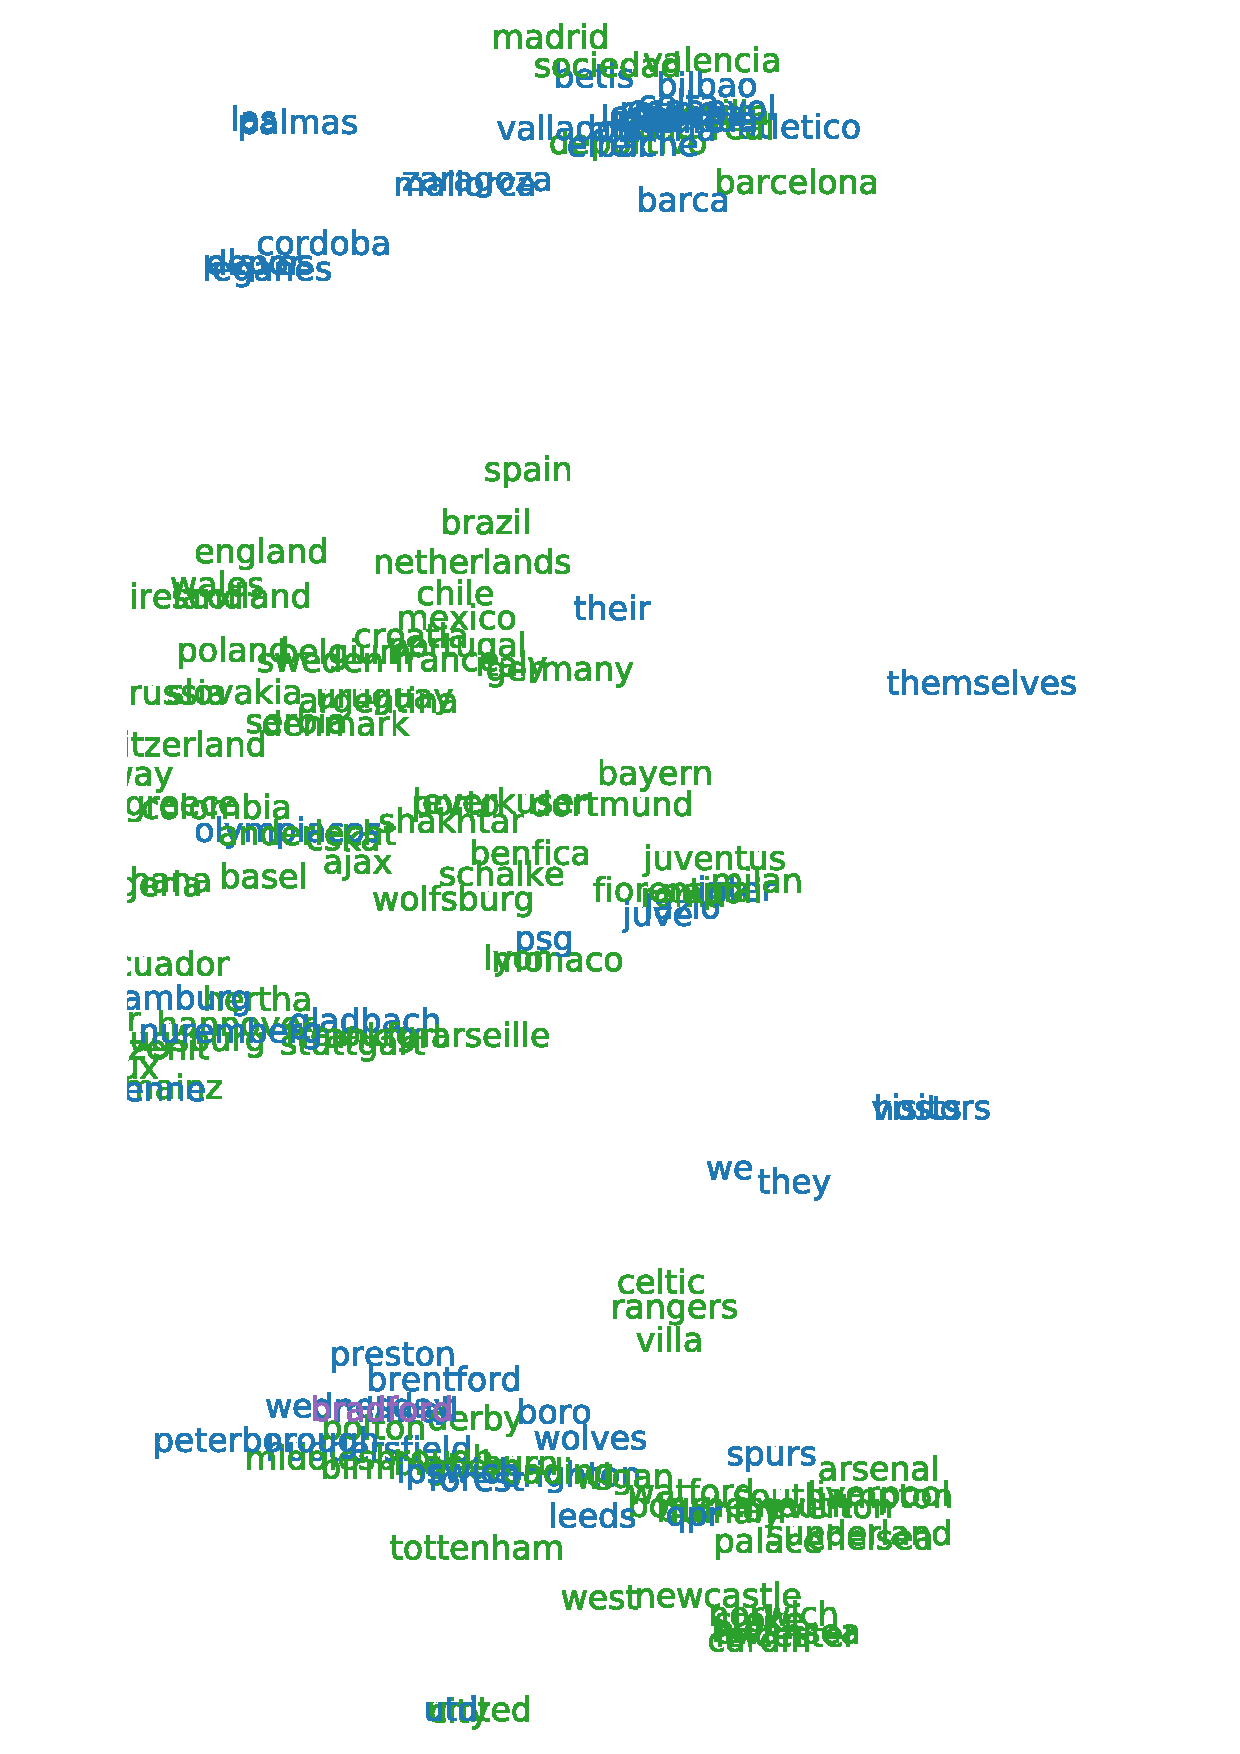
\includegraphics[width=8cm]{figures/tsne_teams.pdf}
\caption{Part of the full t-SNE embedding. The Spanish (top) and English (bottom) teams are shown and clearly separated. This portion can be found towards the centre far right of the whole image on page \pageref{fig:tSNE}.}\label{fig:tsneteams}
\end{wrapfigure}

The underlying data, i.e. the words, are not uniformly distributed across the vector space. This is a result of the granularity of the data itself but also a feature of the underlying language. As a result, similar words lie in a similar direction of the vector space. Since the vector space still has a very high dimensionality, it does not make sense to project the vector space down to two dimensions in the way that this is possible for three dimensions. This will lead to the overlap of many datapoints but more crucially, none of the dimensions of the vector space have a particular meaning. Whereas there is a clear connection between an axis and meaning in physics, such as on a time-position plot, the dimensions of the word vectors collectively contain information. Instead, one has to use more sophisticated methods that preserve the density structure of the data into a lower dimensionality. One such method is to use the t-SNE algorithm \cite{t-SNE}. The abbreviation stands for "t-distributed Stochastic Neighbourhood Embedding". A detailed derivation and explanation of the algorithm can be found in [ibid.] and is not repeated here. The result of applying the algorithm to the dataset is shown in full on page \pageref{fig:tSNE} in the appendix. The words in there are coloured for visual convenience and the clustering of words of similar meaning is visible. The colouring is not complete but should give sufficient guidance to select similar words. 

Interesting parts of the embedding are shown in the following paragraphs. Figure \ref{fig:tsneteams} shows part of the team names; Note how the model successfully separates Spanish league teams (top) and English league teams (bottom). Between these two "clouds", more team names continue towards the center of the embedding. This broader cloud also contains country names, as teams participating in the World Cup. The clear separation of these two areas and the mixture of other clubs and countries can be explained by the relative number of mentions. In its coverage, sportsmole may focus more on the English and Spanish league, so other countries' teams receive less mention and cannot be clearly separated.

The closeness of words does not directly relate to a high similarity score. For dense patches such as the Spanish team names in figure \ref{fig:tsneteams}, the words in a patch have an average similarity score of $0.74\pm0.16$. The similarity to the grouping country Spain varies similarly, $0.77\pm 0.13$. For quite a number of teams in the Spanish team group, the similarity to Spain is as big as their relative similarity. On the other hand, the similarity between Spain and other nations is also very high, so its position on the outset of the nations patch is warranted. In other cases, the reason for the finer structure is unclear. In the same image, the three words "celtic", "ranger" and "villa" have the same similarity to each other as to the logical grouping of English teams just next to them.

\begin{wrapfigure}{r}{6cm}
\vspace{-2cm}
%\hspace{-1cm}
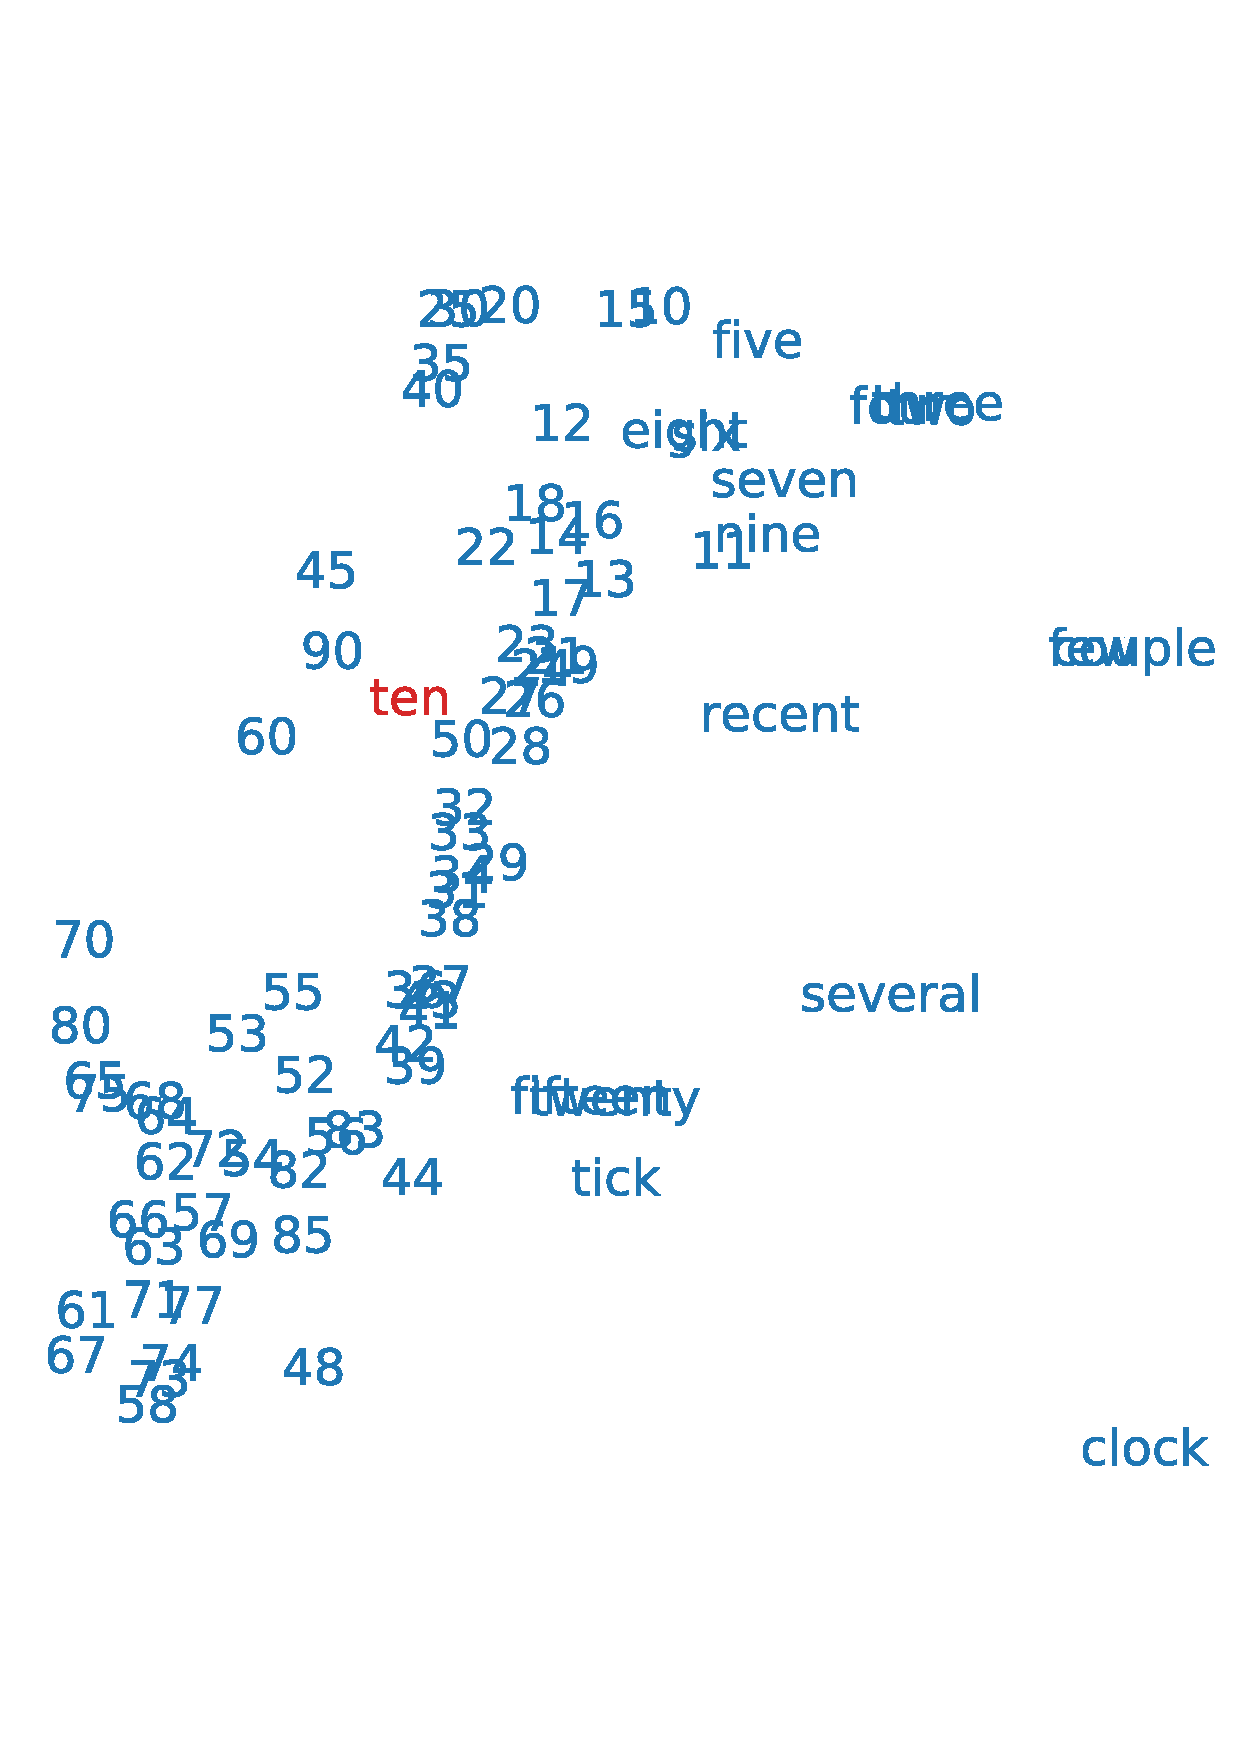
\includegraphics[width=6.5cm]{figures/tsne_numbers.pdf}
\vspace{-2cm}
\caption{Grouping of numbers found in the t-SNE embedding. This part can be found in the upper middle part of the full image.}\label{fig:tsnenumbers}
\end{wrapfigure}

Another corner of the image collects most of the numbers together, as shown in figure \ref{fig:tsnenumbers}. Note how both digits and spelt-out words are collected together. Note that other number related words like "few" and "couple" also appear in vicinity. The word "clock" also appears close in the embedding. Curiously, the numbers increase from top to bottom. All numbers are closely related to each other ($0.69\pm0.18$), but the similarity of each number and its written-out equivalent is low ($0.50 \pm 0.19$) with a large variation. Even more unrelated is the word "clock", despite its depiction nearby, with a similarity of ($0.29\pm0.12$) to all digit numbers. 

The reason for these variations in the similarity are rooted in the text corpus, where digit numbers and written numbers are presumably used in different context. In football, numbers refer both to minutes and times but also to players, as each player has an associated number. Players don't appear to be referred to by number, as table \ref{tab:playernumbers} shows. Within the first five closest word vectors, the correct player number is not found.

\begin{table}[hb]\hspace{-1cm}
\footnotesize
\begin{tabular}{r l c c c c c}
player & correct\hspace{-20pt} & \multicolumn{5}{c}{closest vectors}\\\hline
Messi & 10 & $\begin{matrix} \text{8} \\ 0.268 \end{matrix}$  & $\begin{matrix} \text{3} \\ 0.261 \end{matrix}$  & $\begin{matrix} \text{9} \\ 0.220 \end{matrix}$  & $\begin{matrix} \text{6} \\ 0.211 \end{matrix}$  & $\begin{matrix} \text{51} \\ 0.070 \end{matrix}$\\
Ronaldo & 7 & $\begin{matrix} \text{8} \\ 0.342 \end{matrix}$  & $\begin{matrix} \text{9} \\ 0.342 \end{matrix}$  & $\begin{matrix} \text{3} \\ 0.292 \end{matrix}$  & $\begin{matrix} \text{6} \\ 0.247 \end{matrix}$  & $\begin{matrix} \text{4} \\ 0.194 \end{matrix}$\\
Kane & 18 & $\begin{matrix} \text{7} \\ 0.312 \end{matrix}$  & $\begin{matrix} \text{6} \\ 0.279 \end{matrix}$  & $\begin{matrix} \text{3} \\ 0.255 \end{matrix}$  & $\begin{matrix} \text{2} \\ 0.225 \end{matrix}$  & $\begin{matrix} \text{1} \\ 0.225 \end{matrix}$\\
Gerrard & 8 & $\begin{matrix} \text{7} \\ 0.308 \end{matrix}$  & $\begin{matrix} \text{6} \\ 0.283 \end{matrix}$  & $\begin{matrix} \text{3} \\ 0.266 \end{matrix}$  & $\begin{matrix} \text{2} \\ 0.264 \end{matrix}$  & $\begin{matrix} \text{2} \\ 0.264 \end{matrix}$\\
Cahill & 17 & $\begin{matrix} \text{8} \\ 0.305 \end{matrix}$  & $\begin{matrix} \text{7} \\ 0.305 \end{matrix}$  & $\begin{matrix} \text{3} \\ 0.281 \end{matrix}$  & $\begin{matrix} \text{0} \\ 0.277 \end{matrix}$  & $\begin{matrix} \text{4} \\ 0.248 \end{matrix}$\\
Terry & 26 & $\begin{matrix} \text{6} \\ 0.385 \end{matrix}$  & $\begin{matrix} \text{7} \\ 0.385 \end{matrix}$  & $\begin{matrix} \text{3} \\ 0.357 \end{matrix}$  & $\begin{matrix} \text{4} \\ 0.357 \end{matrix}$  & $\begin{matrix} \text{5} \\ 0.331 \end{matrix}$\\\hline
\end{tabular}
\begin{tabular}{r l c c c c c}
player & correct\hspace{-20pt} & \multicolumn{5}{c}{closest vectors}\\\hline
Mertesacker & 4 & $\begin{matrix} \text{7} \\ 0.346 \end{matrix}$  & $\begin{matrix} \text{3} \\ 0.331 \end{matrix}$  & $\begin{matrix} \text{5} \\ 0.257 \end{matrix}$  & $\begin{matrix} \text{6} \\ 0.257 \end{matrix}$  & $\begin{matrix} \text{1} \\ 0.257 \end{matrix}$\\
Ramsey & 8 & $\begin{matrix} \text{6} \\ 0.327 \end{matrix}$  & $\begin{matrix} \text{3} \\ 0.297 \end{matrix}$  & $\begin{matrix} \text{5} \\ 0.231 \end{matrix}$  & $\begin{matrix} \text{3} \\ 0.297 \end{matrix}$  & $\begin{matrix} \text{0} \\ 0.254 \end{matrix}$\\
Özil & 11 & $\begin{matrix} \text{7} \\ 0.296 \end{matrix}$  & $\begin{matrix} \text{3} \\ 0.290 \end{matrix}$  & $\begin{matrix} \text{5} \\ 0.270 \end{matrix}$  & $\begin{matrix} \text{4} \\ 0.240 \end{matrix}$  & $\begin{matrix} \text{2} \\ 0.240 \end{matrix}$\\
Ibrahimovic & 9 & $\begin{matrix} \text{7} \\ 0.378 \end{matrix}$  & $\begin{matrix} \text{6} \\ 0.347 \end{matrix}$  & $\begin{matrix} \text{3} \\ 0.336 \end{matrix}$  & $\begin{matrix} \text{2} \\ 0.328 \end{matrix}$  & $\begin{matrix} \text{4} \\ 0.301 \end{matrix}$\\
Schweinsteiger & 31 & $\begin{matrix} \text{6} \\ 0.353 \end{matrix}$  & $\begin{matrix} \text{8} \\ 0.324 \end{matrix}$  & $\begin{matrix} \text{7} \\ 0.353 \end{matrix}$  & $\begin{matrix} \text{4} \\ 0.336 \end{matrix}$  & $\begin{matrix} \text{5} \\ 0.281 \end{matrix}$\\
Pieters & 3 & $\begin{matrix} \text{3} \\ 0.234 \end{matrix}$  & $\begin{matrix} \text{5} \\ 0.153 \end{matrix}$  & $\begin{matrix} \text{7} \\ 0.175 \end{matrix}$  & $\begin{matrix} \text{6} \\ 0.218 \end{matrix}$  & $\begin{matrix} \text{1} \\ 0.234 \end{matrix}$\\\hline
\end{tabular}
\caption{Relation of select players with their player number. Except for Pieters, none of closest vectors hold the correct value nor are the values located very close to the vector.}\label{tab:playernumbers}
\end{table}

This is not only the case for the ten examples given here, but also for the full roster of players. The player numbers are taken from \cite{plnumbers}. The average similarity hovers around zero, with $0.094\pm0.115$ and out of the 520 player/squad number combinations, the correct number is within the five closest vectors a total of 52 times. This can be safely attributed to chance and the necessary information is presumably not present in the text corpus.

Adjectives that appear in the same context are grouped together by the word2vec embedding algorithm. An example of this can be seen in figure \ref{fig:tsnenations}. Here some of the adjectives describing nationality are collected towards the bottom of the cut-out, with other adjectives appearing in a similar context nearby. Again the similarity between the word vectors is rather high ($0.81\pm0.22$). Common to the words here is not so much that they are similar in function but similar in sentence position. For adjectives of national origin, there is a clear functional relationship, but the words located above appear in similar grammatical context and therefore are deemed similar in the word2vec algorithm.

\begin{wrapfigure}{l}{5cm}
\hspace{-1.5cm}
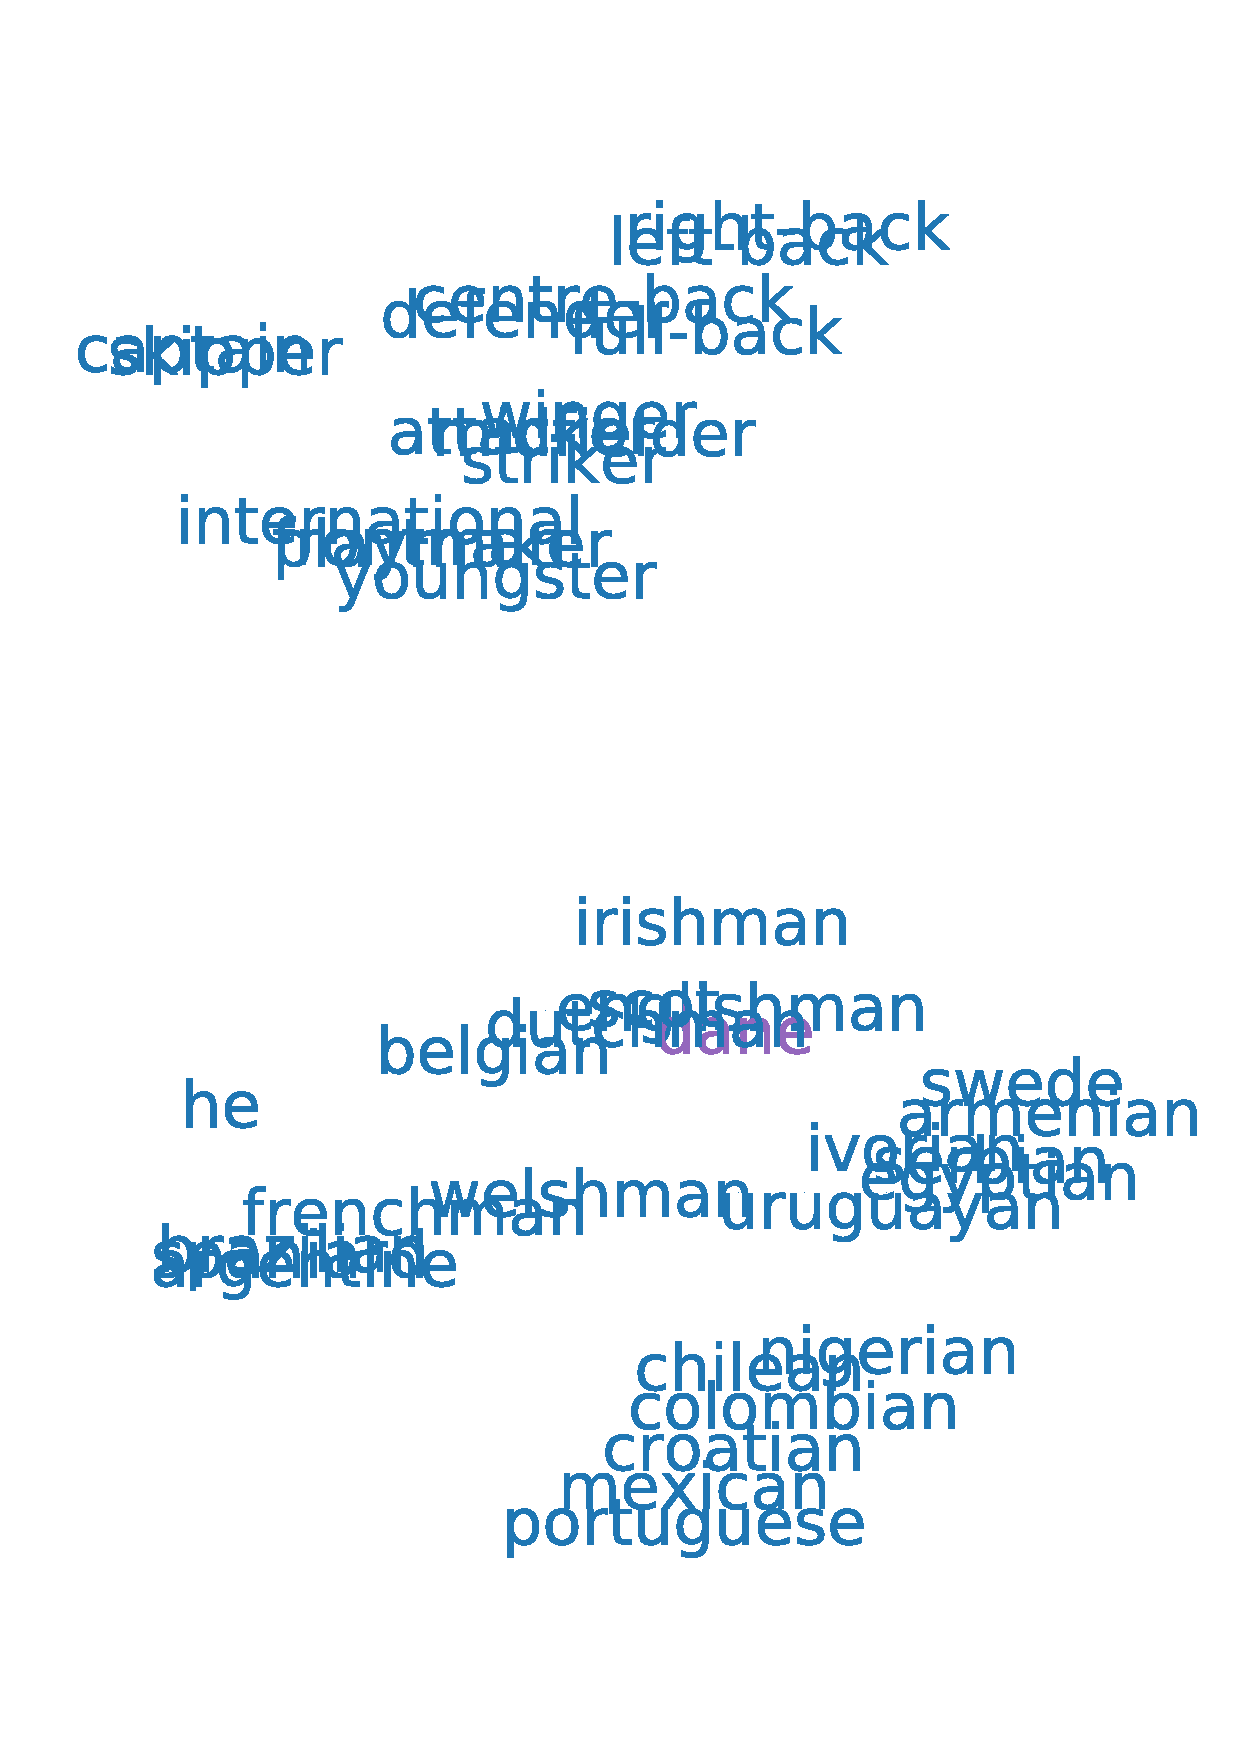
\includegraphics[width=6cm]{figures/tsne_nation_adjectives.pdf}
\caption{Adjectives of nationality together with adjectives describing players. This part can be found towards the top left of the large image, next to the diffuse red player name cloud.}\label{fig:tsnenations}
\end{wrapfigure}

From the observations made here, the diagram of word relationships generally resembles the similarity seen between different words, i.e. words that are located close to each other in the final two-dimensional diagram. This corresponds to the difficulty of mapping a high-dimensional space down to just two dimensions, where the similarity measure just gives an angle between two vectors but does not tell in which dimensions a similarity is present. The strength of the t-SNE algorithm is the creation of a diagram that clearly and quickly reveals which words are related to each other. The two-dimensional embedding therefore resembles the coarse structure of the word2vec space. 

\begin{wrapfigure}{r}{6cm}
\includegraphics[width=6cm]{figures/Messi_similarity.png}
\caption{Illustration of a similarity query for the player name "Messi". The 20 closest vectors are shown. The distance from the central point is one minus the similarity (which is on a scale from $1$ to $-1$), so more similar vectors are located closer to the target vector. Colors do not carry a meaning.}\label{fig:messisim}
\end{wrapfigure}

While the corpus at large brings its own interesting points of study, individual players can also be queried. The word2vec corpus can show similar vectors together with an indication of similarity. Examples of such similarity queries are illustrated in figure \ref{fig:messisim}. The query returns players that play in similar positions \cite{sumpter2}. and similar performance. At a greater distance, but still related, the word "argentine" indicates a common synonym for Messi, such as in the replacement "the Argentine". Note also that many of the names of other players have a background in Spanish or Portuguese, indicating another axis of similarity. This and other queries show the strength of the word2vec word embedding, with easy word similarity queries and generally valid results. Further queries are shown in table \ref{tab:moresim}, negative queries in table \ref{tab:dissim}. Note how words that are unique in their meaning, such as "goal", have no close (similar) vector, whereas the space around player names is densely populated, as seen by the example of the player name "Ronaldo". For country names, the picture is similar, all similar vectors are located very close to each other, indicated in the example by "Sweden". The same is true for cities, as exemplified by word vectors located close to "Stockholm". Keeper shows the synonym goalkeeper as a nearby word vector and the list of names afterwards indicate players that take the keeper role.

\begin{table}[hb]
\scriptsize
\hspace{-0.2cm}
\begin{tabular}{r|c c c c c c c c}
Goal
 & $\begin{matrix}\text{defeat}\\0.419\end{matrix}$
 & $\begin{matrix}\text{leg}\\0.394\end{matrix}$
 & $\begin{matrix}\text{overhead}\\0.391\end{matrix}$
 & $\begin{matrix}\text{bicycle}\\0.379\end{matrix}$
 & $\begin{matrix}\text{victory}\\0.377\end{matrix}$
  & $\begin{matrix}\text{target}\\0.377\end{matrix}$
 & $\begin{matrix}\text{spot}\\0.358\end{matrix}$
 & $\begin{matrix}\text{post}\\0.354\end{matrix}$
\\\hline
Foul
 & $\begin{matrix}\text{lunge}\\0.756\end{matrix}$
 & $\begin{matrix}\text{trip}\\0.733\end{matrix}$
 & $\begin{matrix}\text{handball}\\0.728\end{matrix}$
 & $\begin{matrix}\text{tug}\\0.718\end{matrix}$
 & $\begin{matrix}\text{shove}\\0.705\end{matrix}$
 & $\begin{matrix}\text{challenge}\\0.676\end{matrix}$
 & $\begin{matrix}\text{tackle}\\0.656\end{matrix}$
 & $\begin{matrix}\text{simulation}\\0.619\end{matrix}$
\\\hline
Team
 & $\begin{matrix}\text{side}\\0.787\end{matrix}$
 & $\begin{matrix}\text{supporters}\\0.656\end{matrix}$
 & $\begin{matrix}\text{manager}\\0.629\end{matrix}$
 & $\begin{matrix}\text{outfit}\\0.605\end{matrix}$
 & $\begin{matrix}\text{record}\\0.558\end{matrix}$
 & $\begin{matrix}\text{club}\\0.546\end{matrix}$
 & $\begin{matrix}\text{fans}\\0.528\end{matrix}$
 & $\begin{matrix}\text{champions}\\0.524\end{matrix}$
\\\hline
Ronaldo
 & $\begin{matrix}\text{benzema}\\0.894\end{matrix}$
 & $\begin{matrix}\text{bale}\\0.872\end{matrix}$
 & $\begin{matrix}\text{griezmann}\\0.847\end{matrix}$
 & $\begin{matrix}\text{messi}\\0.823\end{matrix}$
 & $\begin{matrix}\text{neymar}\\0.786\end{matrix}$
 & $\begin{matrix}\text{isco}\\0.784\end{matrix}$
 & $\begin{matrix}\text{modric}\\0.783\end{matrix}$
 & $\begin{matrix}\text{morata}\\0.760\end{matrix}$
 \\\hline
Sweden
 & $\begin{matrix}\text{denmark}\\0.896\end{matrix}$
 & $\begin{matrix}\text{italy}\\0.885\end{matrix}$
 & $\begin{matrix}\text{porto}\\0.880\end{matrix}$
 & $\begin{matrix}\text{france}\\0.879\end{matrix}$
 & $\begin{matrix}\text{belgium}\\0.878\end{matrix}$
 & $\begin{matrix}\text{portugal}\\0.874\end{matrix}$
 & $\begin{matrix}\text{poland}\\0.871\end{matrix}$
 & $\begin{matrix}\text{russia}\\0.870\end{matrix}$
 \\\hline
Keeper
 & $\begin{matrix}\text{goalkeeper}\\0.808\end{matrix}$
 & $\begin{matrix}\text{mignolet}\\0.781\end{matrix}$
 & $\begin{matrix}\text{lloris}\\0.777\end{matrix}$
 & $\begin{matrix}\text{szczesny}\\0.768\end{matrix}$
 & $\begin{matrix}\text{begovic}\\0.764\end{matrix}$
 & $\begin{matrix}\text{speroni}\\0.754\end{matrix}$
 & $\begin{matrix}\text{guzan}\\0.754\end{matrix}$
 & $\begin{matrix}\text{schmeichel}\\0.752\end{matrix}$
 \\\hline
Attack
 & $\begin{matrix}\text{counter-attack}\\0.660\end{matrix}$
 & $\begin{matrix}\text{counter}\\0.622\end{matrix}$
 & $\begin{matrix}\text{move}\\0.567\end{matrix}$
 & $\begin{matrix}\text{threat}\\0.558\end{matrix}$
 & $\begin{matrix}\text{break}\\0.555\end{matrix}$
 & $\begin{matrix}\text{launch}\\0.520\end{matrix}$
 & $\begin{matrix}\text{counterattack}\\0.518\end{matrix}$
 & $\begin{matrix}\text{charge}\\0.485\end{matrix}$
 \\\hline
Stockholm
 & $\begin{matrix}\text{naples}\\0.700\end{matrix}$
 & $\begin{matrix}\text{bydgoszcz}\\0.673\end{matrix}$
 & $\begin{matrix}\text{andalusia}\\0.668\end{matrix}$
 & $\begin{matrix}\text{catalonia}\\0.647\end{matrix}$
 & $\begin{matrix}\text{maryland}\\0.647\end{matrix}$
 & $\begin{matrix}\text{glasgow}\\0.636\end{matrix}$
 & $\begin{matrix}\text{bangkok}\\0.636\end{matrix}$
 & $\begin{matrix}\text{florence}\\0.632\end{matrix}$
 \end{tabular}
\caption{Example word similarity queries from the generated word2vec database. The word is indicated at the top, the similarity on a scale from one (coincides) to minus one (completely opposite) is indicated below. Note how player names generally create other player names with high similarity. The eight most similar words are shown.}\label{tab:moresim}
\end{table}

\begin{table}
\scriptsize
\hspace{-1.5cm}
\begin{tabular}{r|c c c c c c c c}
$-$Goal
& $ \begin{matrix} \text{joins} \\ 0.381 \end{matrix}$
& $ \begin{matrix} \text{enters} \\ 0.373 \end{matrix}$
& $ \begin{matrix} \text{demands} \\ 0.367 \end{matrix}$
& $ \begin{matrix} \text{toward} \\ 0.362 \end{matrix}$
& $ \begin{matrix} \text{artificial} \\ 0.358 \end{matrix}$
& $ \begin{matrix} \text{flattens} \\ 0.355 \end{matrix}$
& $ \begin{matrix} \text{featuring} \\ 0.348 \end{matrix}$
& $ \begin{matrix} \text{cardnow} \\ 0.347 \end{matrix}$
\\\hline
$-$Foul
& $ \begin{matrix} \text{lacks} \\ 0.352 \end{matrix}$
& $ \begin{matrix} \text{around} \\ 0.345 \end{matrix}$
& $ \begin{matrix} \text{entire} \\ 0.337 \end{matrix}$
& $ \begin{matrix} \text{lacked} \\ 0.322 \end{matrix}$
& $ \begin{matrix} \text{onto} \\ 0.304 \end{matrix}$
& $ \begin{matrix} \text{complexion} \\ 0.300 \end{matrix}$
& $ \begin{matrix} \text{carousel} \\ 0.288 \end{matrix}$
& $ \begin{matrix} \text{cliché} \\ 0.286 \end{matrix}$
\\\hline
$-$Team
& $ \begin{matrix} \text{right-hand} \\ 0.474 \end{matrix}$
& $ \begin{matrix} \text{left-hand} \\ 0.460 \end{matrix}$
& $ \begin{matrix} \text{rescues} \\ 0.456 \end{matrix}$
& $ \begin{matrix} \text{well-positioned} \\ 0.432 \end{matrix}$
& $ \begin{matrix} \text{wrong} \\ 0.428 \end{matrix}$
& $ \begin{matrix} \text{outmuscles} \\ 0.413 \end{matrix}$
& $ \begin{matrix} \text{falls} \\ 0.405 \end{matrix}$
& $ \begin{matrix} \text{misdirected} \\ 0.399 \end{matrix}$
\\\hline
$-$Ronaldo
& $ \begin{matrix} \text{hounding} \\ 0.599 \end{matrix}$
& $ \begin{matrix} \text{outnumber} \\ 0.583 \end{matrix}$
& $ \begin{matrix} \text{pressurising} \\ 0.520 \end{matrix}$
& $ \begin{matrix} \text{bombarding} \\ 0.515 \end{matrix}$
& $ \begin{matrix} \text{playmaking} \\ 0.505 \end{matrix}$
& $ \begin{matrix} \text{harrying} \\ 0.503 \end{matrix}$
& $ \begin{matrix} \text{isbookedfor} \\ 0.493 \end{matrix}$
& $ \begin{matrix} \text{changeit} \\ 0.492 \end{matrix}$
\\\hline
$-$Sweden
& $ \begin{matrix} \text{loanee} \\ 0.495 \end{matrix}$
& $ \begin{matrix} \text{skipper} \\ 0.479 \end{matrix}$
& $ \begin{matrix} \text{over-play} \\ 0.474 \end{matrix}$
& $ \begin{matrix} \text{penalise} \\ 0.474 \end{matrix}$
& $ \begin{matrix} \text{substitutionfor} \\ 0.468 \end{matrix}$
& $ \begin{matrix} \text{foil} \\ 0.459 \end{matrix}$
& $ \begin{matrix} \text{hounding} \\ 0.445 \end{matrix}$
& $ \begin{matrix} \text{enner} \\ 0.441 \end{matrix}$
\\\hline
$-$Keeper
& $ \begin{matrix} \text{involving} \\ 0.536 \end{matrix}$
& $ \begin{matrix} \text{featuring} \\ 0.525 \end{matrix}$
& $ \begin{matrix} \text{fells} \\ 0.523 \end{matrix}$
& $ \begin{matrix} \text{xabi} \\ 0.452 \end{matrix}$
& $ \begin{matrix} \text{alongside} \\ 0.450 \end{matrix}$
& $ \begin{matrix} \text{talented} \\ 0.447 \end{matrix}$
& $ \begin{matrix} \text{aleix} \\ 0.443 \end{matrix}$
& $ \begin{matrix} \text{cesc} \\ 0.441 \end{matrix}$
\\\hline
$-$Attack
& $ \begin{matrix} \text{stooped} \\ 0.410 \end{matrix}$
& $ \begin{matrix} \text{downward} \\ 0.403 \end{matrix}$
& $ \begin{matrix} \text{int} \\ 0.391 \end{matrix}$
& $ \begin{matrix} \text{ripples} \\ 0.389 \end{matrix}$
& $ \begin{matrix} \text{steers} \\ 0.382 \end{matrix}$
& $ \begin{matrix} \text{plants} \\ 0.377 \end{matrix}$
& $ \begin{matrix} \text{guided} \\ 0.375 \end{matrix}$
& $ \begin{matrix} \text{sufficient} \\ 0.371 \end{matrix}$
\\\hline
$-$Stockholm
& $ \begin{matrix} \text{in} \\ 0.342 \end{matrix}$
& $ \begin{matrix} \text{through} \\ 0.273 \end{matrix}$
& $ \begin{matrix} \text{inside} \\ 0.270 \end{matrix}$
& $ \begin{matrix} \text{out} \\ 0.245 \end{matrix}$
& $ \begin{matrix} \text{easy} \\ 0.241 \end{matrix}$
& $ \begin{matrix} \text{happy} \\ 0.241 \end{matrix}$
& $ \begin{matrix} \text{about} \\ 0.235 \end{matrix}$
& $ \begin{matrix} \text{comfortable} \\ 0.233 \end{matrix}$
\end{tabular}
\caption{Example word similarity queries from the generated word2vec database, for the negative word vector. These are the 8 most dissimilar words for each word. Spelling as in original.}\label{tab:dissim}
\end{table}


Similarly, the word2vec database presents more detailed descriptions for words, such as "foul", where most of the actions described here would lead to a foul. There can also be spelling variations, as seen in the words similar to "attack". "counter-attack" and "counterattack" mean the same thing (the similarity between the words is only $0.800$). "Counter-attack" describes an opposing move, but it reasonably can appear in the context of "attack". The list of similar words is not perfect however. "Porto" does not belong into the list of countries presented as similar to the word "Sweden". The words presented here indicate a good quality of the generated word vectors. A more extensive overview of 70 randomly chosen words and their similarities is shown in figure \ref{fig:simmatrix}. The plot there is visually dominated by a generally high similarity between words (red squares) dissected by apparent lines of words with lower similarity to most other words (blue squares). In particular the words "defensively", "throw", "schalke" and "45" have a generally negative similarity to the words shown here.

\begin{figure}[hbt]
\includegraphics[width=0.5\textwidth]{figures/simmat_spanish_teams.pdf}
\includegraphics[width=0.5\textwidth]{figures/simmat_english_teams.pdf}
\caption{Similarity matrix for the spanish (left) and english (right) team names, as found in part of figure \ref{fig:tsneteams}. Words that have a general meaning outside of a team name are excluded, such as "city" or "town". Note that the two matrixes use a different colour scale.}\label{fig:simmatrixspain}
\end{figure}

The vectors shown in the t-SNE excerpts can be examined examined for their individual similarity queries. For the spanish teams, the picture looks like expected, a high similarity between all team names (Note the change in scale). The similarity matrix is shown on the left side of figure \ref{fig:simmatrixspain}. The word "athletic" in "Athletic Madrid" is presumably captured by its meaning as an adjective. The same may also be true for "real", but the dissimilarity with "vigo", coming the team name "Celta Vigo" is unexpected. For the English teams shown in the right side of figure \ref{fig:simmatrixspain}, the matrix is also quite varied, where several team names appear to be unaligned with the majority of the team names. These names, "Hove", "Crystal", "Manchester", "Hotspur" and "Bromwich" should generally appear only in the context or part of team names. It appears that either these words are dominated by another meaning or that the full team name is not always used. The latter is true in particular for the teams of Manchester, Manchester City and Manchester United, that have a plethora of abbreviations and nicknames.

The numbers as found the t-SNE diagram excerpt shown in figure \ref{fig:tsnenumbers} show a predictable yet interesting pattern. They appear to be very similar in small blocks. The small digit numbers from 0 to 9 show a very high similarity but a lower one to numbers beyond that and their written counterparts. Digit numbers from 10 to 86 are also similar with the notable exception of 46. For the written out words, the pattern repeats, with higher similarity for numbers between one and nine, and ten to twenty but a lower similarity between the two sets. This could represent a use in different context.

\begin{figure}[hbt]
\includegraphics{figures/simmat_numbers.pdf}
\caption{Similarity matrix for selected numbers, both in digit form and written out. For the latter, the missing words do not appear in the dataset.}\label{fig:simmatrixnumbers}
\end{figure}

 This quality cannot be quantised because the relationship between words themselves and to the word vectors is not well understood. In fact, what exactly constitutes a similar word is subject to debate \cite{learningwv}. Based on these and other queries, it is assumed that the word2vec model sufficiently captures similarities in the text. The model will be used again in chapter \ref{cha:autogen}.

\begin{figure}
\includegraphics{figures/similarity_matrix.pdf}
\caption{Similarity measures for 50 random words of the corpus, on a similarity scale between $-0.7$ and $0.7$. Since the similarity measure is symmetric, only half of the matrix is shown. Values on the diagonal are set to zero.}\label{fig:simmatrix}
\end{figure}

\paragraph{Side note}
From the similarity exploration in table \ref{tab:moresim}, the size of the vector space becomes apparent. A similarity value of 0.5 corresponds to an angle of 60 degrees, i.e. a cone with a central angle~(!) around the vector. In a humanly conceivable three-dimensional vector space, 120${}^\circ$ patches would lead to an overlap with just 4 patches. As the dimension of the space grows, more and more patches can be added of equal opening angle without effectively covering the space. While the surface area of an $n$-sphere goes to zero as $n\to\infty$, since the surface of a $n$-sphere is expressed as
\begin{align}
\Omega_{S^n} = \frac{2^{\frac{n+1}2}}{\Gamma(\frac{n+1}2)}
\end{align}
The steradian for angle $\theta$ in $n$ dimensions is expressed as \cite{mathstack}:
\begin{align}
\Omega_n(\theta) = \Omega_{S^n} \int_0^\theta ~\text{d}\phi \sin^n(\phi)
\end{align}
This expression tends to zero for large $n$ because of the $\Omega_{S^n}$ prefactor. In turn this means that there can be many patches of opening angle $\theta$ before the space is covered. The space of the word vectors can be considered sparse. Measuring similarity to a random vector on the surface of the $n$-sphere created with Marsaglia's algorithm \cite{marsaglia} returns an average similarity to the next vector of 0.35, corresponding to a 70 degree central angle, 140${}^\circ$ opening angle. It is difficult to relate this to a real-world concept, what this means is that the space available in 100 dimensions is not appreciably covered by the 15000 vectors available here.

%\begin{itemize}
%\item {\color{green} distribution of comment length}
%\item {\color{green}distribution of words (power law, word frequency)}
%\item {\color{green}Take out half of goal because it is machine written}
%\item {\color{orange}word2vec and why}
%\item {\color{red}t-SNE diagrams}
%\item racism through adjectives
%\item pesky low-frequency words
%\item text generation via LSTM
%\end{itemize}



\chapter{Bias in writing}\label{cha:bias}

A further area of analysis is a possible bias of the author towards a particular player, team or player's race. In particular, are some players described with particular attributes more often than other players? There are two immediate ways to approach this question, both of which are explored below. The first is to look at the adjectives and adverbs associated with a player or team, the other to approach it via the mathematical understanding generated by the word2vec algorithm.

In order to find associated attributes, the adjectives and adverbs have to be identified. Within the NLTK framework \cite{nltk}, there exists an algorithm for automatically identifying adjectives and adverbs, based on word position within the sentence and a dictionary look-up. Using this algorithm, each word in the sentence is identified with its grammatical function, such as noun, verb, adjective or adverb. Each token in a comment that is identified as a adjective or adverb is associated with one or more players in the same comment. This collection is run over the whole commentary text.

There are a number of draw-backs to this approach, in particular it neglects a direct identification of an adjective with the player or of an adverb with the verb action of the player. Building such an identification on an automatic basis would require significantly more work, hence this slightly crude approximation is taken. The associated tokens are slightly over-counted, but the distribution of adjectives associated with a particular player should not change significantly if the encounters between players is assumed to be sufficiently random.

\section{Randomness and limits thereof}

Sufficiently random here means the following: Suppose a player with a bias gets mentioned in a comment together with a player without a bias. In the next comment, the player with bias will again match up against an unbiased one, retaining the bias. On the other hand, the unbiased players will have sufficiently low encounter rates that their own distribution of associated words is only marginally skewed.

This constraint of sufficient randomness can be interpreted as a constraint on the number of people that exhibit a bias. Take the set of players as $A$. All elements in this set are indistinguishable except for the fact that some are subject to a bias. This can be interpreted mathematically as grouping into two distinct populations,
\begin{align}
x&\in B\subset A\\
x&\in A \backslash B
\end{align} 
where $B$ contains all individuals subject to a bias, $A\backslash B$ those without a bias. Consider random pairings of elements,
\begin{align}
x_1, x_2 \in A
\end{align}
These represent the players in the commentary. If one or both of these elements in the pairing are in a subset $x_1 \vee x_2 \in B\subset A$, they both get a mark. This pairing represents biased players appearing together with "normal" players. If $x_1 \wedge x_2 \in A\backslash B$, they do not get a tag. How many players are tagged and how does a cutoff need to be set in order to avoid mis-classifying players? For a high enough count of pairwise count, the separation between $A$ and $B$ will be clean because there are enough counts of pairs $x_1, x_2\in A\backslash B$. The baseline incidence there is trivially $\#B / \# A$. Where the number of pairs is not high enough, one can get an idea of how the baseline incidence via a simulation.

For the simulation, take $A$ to hold 100 elements and take 1000 pairings. This gives an average of 20 pairings for each element. If an element is special, give a tag to both members of the pairing, otherwise just increase their count. The number of tags divided by the number times the element appeared in a pair is shown in figure \ref{fig:pairings}, for varying numbers of elements $x \in B \subset A$.

\begin{figure}\centering
\includegraphics[width=10cm]{figures/random_pairings.png}
\caption{The incidence rate of tags for random pairings, for different values of tagged members. Tagged members are all arranged starting from the left.}\label{fig:pairings}
\end{figure}

From the plot it can be seen that the incidence rate is subject to random fluctuation. If one percent of the elements $x\in A$ carry a tag, a confidence interval of $p<0.05$ or $p>0.05$ will lead to the mis-classification of more than 15 individuals. If the incidence rate of biased individuals goes down to 0.1\%, the classification still hits more than ten individuals instead of the one correct one. The actual false-positive rate depends on the number of individuals that receive a bias, the number of individuals and the strength of a bias.

This mathematical analysis presents the extreme case, with a few players that are subject to an extreme bias and many unbiased ones. This is not be expected in the real world, were there will be a slight bias towards or against particular players and not one player solely receiving bias. The interplay of writing bias and the consequences of analysing the text will be subtler, but the analysis here shows the likelihood of false error rates. Grouping players by a common element should dampen the false error rates seen above.

In addition to that, the approach of tagging players still works because comments often enough focus on a single player and the bias is not as clear as assumed in the simulation. The pairings seen in comments are also not fully random. Different teams meet each other twice per season, so there the distribution is uniform. However, different players take different roles, so attackers from one team will rarely interact with attackers from another team, simply because they play in opposite parts of the field.

Since the collection takes all the adjectives and adverbs in the sentence, there will be also a lot of unrelated adjectives in the collection. Hence the results are filtered for a select group of adjectives, shown in table \ref{tab:selectedwords}.

\begin{wraptable}{i}{5.4cm}\centering
\begin{tabular}{c c c}
\hline
bad & poor & frustrated\\
amazing & great & fantastic\\
aggressive & angry & dangerous\\\hline
\end{tabular}
\caption{Words selected for bias analysis}\label{tab:selectedwords}\vspace{-0.5cm}
\end{wraptable}

The $p$-value can be easily found by modeling the association of adjectives with a player in the form of a binomial distribution.\footnote{For numerical stability, the actual calculation is done with a Gaussian distribution approximation. This is justified in cases where the number of expected counts $np>5$ \cite{statsforexp}.}
\begin{align}
p_\text{adj} = \sum_{i=0}^{k_\text{adj}} \begin{pmatrix} n\\i\end{pmatrix} p_\text{adj}^i (1 - p_\text{adj})^{n - i}
\end{align}

\begin{wraptable}{r}{7.5cm}\centering
%\vspace{-10pt}
\scriptsize
\begin{tabular}{r l r l}
Player (\#tags) & Attribute (\#found) & Expected & $p$-value\\\hline
Gayle (867) &great (13) & 4.9 & $0.9998$\\
Murray (982) &great (11) & 4.7 & $0.9982$\\
Ritchie (1102) &dangerous (11) & 5.0 & $0.9966$\\
{\color{gray}Naughton (631)} &{\color{gray}dangerous (12)} & {\color{gray}3.1} & {\color{gray}$0.9999$}\\
{\color{gray}Mcclean (606)} &{\color{gray}poor (11)} & {\color{gray}3.0} & {\color{gray}$0.9999$}\\
Lovren (1575) &dangerous (16) & 10.3 & $0.9614$\\
Smalling (1417) &dangerous (12) & 7.0 & $0.9717$\\
Brunt (1513) &dangerous (14) & 8.9 & $0.9646$\\
Barry (1491) &dangerous (11) & 6.7 & $0.9506$\\
Davis (1350) &poor (12) & 7.3 & $0.9592$\\
Davis (1350) &great (12) & 7.1 & $0.9691$\\
Reid (1260) &dangerous (11) & 5.7 & $0.9872$\\
Moreno (1238) &poor (12) & 6.7 & $0.9800$\\
Shaw (1264) &dangerous (11) & 5.7 & $0.9868$\\
Blind (920) &dangerous (13) & 4.9 & $0.9998$\\
Morrison (1186) &great (11) & 5.7 & $0.9873$\\
Cyne (1413) &great (14) & 8.6 & $0.9672$\\
Vorm (1070) &great (11) & 5.1 & $0.9953$\\\hline
\end{tabular}
\caption{Player-attribute list from the sportsmole dataset ($p>0.95$) based on the selected attributes shown in table \ref{tab:selectedwords}. These are the words that appear more often than expected. Gray lines indicate $np\ll5$, where the Gaussian approximation to the binomial distribution is not valid. These data lines are included for sake of completeness.}\label{tab:pgreater0.95}\vspace{-30pt}
\end{wraptable}

where $n$ is the total number of adjectives of the player and the probability $p_\text{adj}$ is the fraction of the particular adjective over all adjectives, $\frac{N_\text{adj}}{N_\text{total}}$. $k$ is the count of the adjective for that player. The list of found statistical oddities needs to be filtered for words that would indicate a bias. The selected words are shown in table \ref{tab:selectedwords}. Cases where the number of actual found adjectives is less than ten are excluded. The analysis is run over the whole sportsmole and goal.com corpus with the names of all Premier League players of the 2017/18 season \cite{playerlistpl}. Some players are excluded where their names coincide with other meanings, such as "can", "will", "field", "hazard" and "long". In total, there are 844 names of 534 players\footnote{Each element of the players, first, middle and last name counts as one name in the analysis. Commonly the player is referenced by his last name. It appears that quite a lot of (first) names are assigned more than once.} featured in the analysis.

\section{Too many adjectives}

There is a curiously high count of the word "dangerous", especially given that the players tagged this way are known to be defensive \cite{sumpter1}. Otherwise the list is not indicative of a strong bias [ibid.]. This analysis is somewhat hampered by the low number of attributes found and expected. On average, the expected number is five to seven attributes while more than ten were found. This is statistically significant, as indicated by the $p$-value, but due to the low numbers this may still be a random fluctuation.

\begin{wraptable}{l}{8.3cm}\centering
\vspace{-10pt}
\scriptsize%\hspace{-0.8cm}
\begin{tabular}{r l r l}
Nation (\#tags) & Attribute (\#found) & Expected & $p$-value\\\hline
Poland (2796) & great (14) & 8.6 & $0.9666$\\
 Germany (2925) & great (15) & 9.7 & $0.9571$\\
 Germany (2925) & dangerous (16) & 9.7 & $0.9782$\\
 Egypt (2918) & dangerous (14) & 8.5 & $0.9710$\\
 Ghana (2955) & dangerous (15) & 9.2 & $0.9721$\\
 Algeria (2808) & dangerous (25) & 14.6 & $0.9969$\\
 Algeria (2808) & great (12) & 7.4 & $0.9536$\\
 Iceland (2866) & dangerous (18) & 10.7 & $0.9873$\\
 Iceland (2866) & great (13) & 8.2 & $0.9529$\\
 Senegal (2682) & great (15) & 8.9 & $0.9804$\\
 Senegal (2682) & dangerous (12) & 6.7 & $0.9802$\\
 {\color{gray}United States (1187)} & {\color{gray}dangerous (11)} & {\color{gray}2.7} & {\color{gray}$1.0$}\\
 Norway (2071) & great (11) & 5.0 & $0.9962$\\
 Cameroon (1601) & poor (12) & 4.4 & $0.9999$\\
 Croatia (1715) & dangerous (17) & 6.1 & $0.9999$\\
 Croatia (1715) & poor (11) & 4.3 & $0.9993$\\
 DR Congo (3407) & dangerous (23) & 16.3 & $0.9527$\\
 New Zealand (1878) & dangerous (17) & 6.6 & $0.9999$\\
 New Zealand (1878) & poor (11) & 4.7 & $0.9980$\\
 New Zealand (1878) & great (11) & 4.6 & $0.9986$\\\hline
 \end{tabular}
 \caption{List of relationships between players grouped by nation and the respective adjective ($p>0.95$). The list is filtered for the attributes shown in table \ref{tab:selectedwords}. These are the words that appear more often than expected. The data line for the United States has $np\ll5$, so the Gaussian approximation to the binomial distribution is not valid here. It is included for sake of completeness.}\label{tab:nationg0.96}
 \vspace{-20pt}
 \end{wraptable}

The same analysis run with all team names indicates no bias whatsoever (no significant $p$-values) for any word in the dataset. Reasons for this lack may be found in the fact that all team meet each other with the same frequency, so the number of mentions for each team is approximately the same. 

The analysis can be repeated by grouping players by their country of origin. High $p$-values here would indicate a bias towards players from a particular background. This excludes players who have changed their nationality and now live their life in another country, but still have their roots in another one, at least as far as the writer is concerned.

For many countries of origin, there are many players. This is the case in particular for England, France and a number of other European countries. The nations of origin shown in table \ref{tab:nationg0.96} feature only a few players. For countries in Africa such as Ghana, Algeria, Senegal, Cameroon and the Democratic Republic of Congo (DR Congo), the word "dangerous" appears often in context with players from these countries. The common denominator for players from these countries is their origin in Africa.

The players from these countries do not appear in the individual player tags, table \ref{tab:pgreater0.95}. This indicates an aggregate effect that is lost in the individual player's data. The tag "dangerous" that appears very often may be attached to a player by a description of the player actions themselves (<player> makes a dangerous move towards the goal) or by stopping an action by somebody else (<player> steps up and block a dangerous shot from across the field). The latter sentence construction may be the reason for the high incidence for defensive players. 

If one assumes that the players from the African countries are distributed evenly across the team positions and are equally active and passive, the found effect may indicate a bias of the writer. However the data is by far not detailed enough and the searching mechanism too coarse to make a meaningful indication whether a bias actually exists.

\begin{table}
\hspace{-0.8cm}
\begin{minipage}[t]{8cm}
\scriptsize\vspace{0pt}
\begin{tabular}{r l r l}
Player (\#tags) & Attribute (\#found) & Expected & $p$-value\\\hline
Nathan (16461) & poor (90) & 339.4 & $0.0$\\
Nathan (16461) & bad (14) & 229.9 & $0.0$\\
Nathan (16461) & great (77) & 279.3 & $0.0$\\
Nathan (16461) & dangerous (99) & 338.4 & $0.0$\\
Jack (194916) & great (1024) & 43982 & $0.0$\\
Jack (194916) & dangerous (923) & 37363 & $0.0$\\
Jack (194916) & fantastic (201) & 44069 & $0.0$\\
Jack (194916) & poor (890) & 39751 & $0.0$\\
Jack (194916) & bad (211) & 41045 & $0.0$\\
Jack (194916) & frustrated (61) & 52610 & $0.0$\\
Jack (194916) & amazing (17) & 44778 & $0.0$\\
Jack (194916) & angry (13) & 32486 & $0.0$\\
Richarlison (19852) & great (67) & 293.1 & $0.0$\\
Richarlison (19852) & bad (24) & 475.4 & $0.0$\\
Richarlison (19852) & dangerous (82) & 338.0 & $0.0$\\
Richarlison (19852) & poor (73) & 332.0 & $0.0$\\
Zanka (7374) & dangerous (40) & 61.2 & $0.0030$\\
Zanka (7374) & great (33) & 53.6 & $0.0023$\\
Zanka (7374) & fantastic (11) & 91.2 & $0.0$\\
Zanka (7374) & poor (28) & 47.3 & $0.0024$\\
César (26986) & great (107) & 636.3 & $0.0$\\
César (26986) & dangerous (147) & 823.9 & $0.0$\\
César (26986) & poor (131) & 810.1 & $0.0$\\
César (26986) & bad (25) & 673.3 & $0.0$\\
César (26986) & fantastic (23) & 698.2 & $0.0$\\
Kevin (41004) & dangerous (249) & 2120 & $0.0$\\
Kevin (41004) & great (184) & 1662 & $0.0$\\
Kevin (41004) & poor (164) & 1540 & $0.0$\\
Kevin (41004) & bad (44) & 1800 & $0.0$\\
Kevin (41004) & fantastic (44) & 2029 & $0.0$\\
de (8807) & great (42) & 81.5 & $0.0$\\
de (8807) & dangerous (65) & 118.9 & $0.0$\\
de (8807) & poor (29) & 58.5 & $0.0$\\
Abdoulaye (28397) & great (121) & 757.2 & $0.0$\\
Abdoulaye (28397) & poor (154) & 1002 & $0.0$\\
Abdoulaye (28397) & bad (29) & 821.8 & $0.0$\\
Abdoulaye (28397) & dangerous (133) & 784.3 & $0.0$\\
Abdoulaye (28397) & fantastic (24) & 766.6 & $0.0$\\
Shane (10763) & poor (53) & 130.7 & $0.0$\\
Shane (10763) & bad (14) & 150.4 & $0.0$\\
Shane (10763) & great (67) & 158.9 & $0.0$\\
Shane (10763) & fantastic (17) & 205.8 & $0.0$\\
Shane (10763) & dangerous (51) & 114.0 & $0.0$\\
Pablo (11628) & poor (54) & 143.9 & $0.0$\\
Pablo (11628) & great (56) & 143.5 & $0.0$\\
Pablo (11628) & dangerous (66) & 159.4 & $0.0$\\
Pablo (11628) & bad (11) & 127.6 & $0.0$\\
Joe (13137) & dangerous (74) & 201.9 & $0.0$\\
Joe (13137) & great (54) & 156.3 & $0.0$\\
Joe (13137) & poor (57) & 171.6 & $0.0$\\
Joe (13137) & bad (13) & 170.5 & $0.0$\\
Ashley (5220) & bad (17) & 88.5 & $0.0$\\
Matt (9997) & fantastic (13) & 146.2 & $0.0$\\
Matt (9997) & great (58) & 127.7 & $0.0$\\
Matt (9997) & dangerous (47) & 97.5 & $0.0$\\
Matt (9997) & poor (45) & 103.1 & $0.0$\\
Bernardo (6664) & great (33) & 48.4 & $0.0129$\\
Bernardo (6664) & dangerous (46) & 63.6 & $0.0131$\\
Bernardo (6664) & poor (21) & 32.0 & $0.0250$\\
Wilfried (7163) & poor (37) & 60.7 & $0.0011$\\
Wilfried (7163) & dangerous (38) & 56.5 & $0.0067$\\
Wilfried (7163) & great (25) & 39.4 & $0.0104$\\\hline
\end{tabular}
\end{minipage}
\begin{minipage}[t]{8cm}
\scriptsize\vspace{0pt}
\begin{tabular}{r l r l}
Player(\#tags) & Attribute (\# found) & Expected & $p$-value\\\hline
Netherlands (16461) & poor (90) & 339.5 & $0.0$\\
Netherlands (16461) & bad (14) & 230.0 & $0.0$\\
Netherlands (16461) & great (77) & 279.3 & $0.0$\\
Netherlands (16461) & dangerous (99) & 338.5 & $0.0$\\
England (194916) & great (1024) & 43983 & $0.0$\\
England (194916) & dangerous (923) & 37364 & $0.0$\\
England (194916) & fantastic (201) & 44070 & $0.0$\\
England (194916) & poor (890) & 39751 & $0.0$\\
England (194916) & bad (211) & 41045 & $0.0$\\
England (194916) & frustrated (61) & 52610 & $0.0$\\
England (194916) & amazing (17) & 44778 & $0.0$\\
England (194916) & angry (13) & 32486 & $0.0$\\
Brazil (19852) & great (67) & 293.1 & $0.0$\\
Brazil (19852) & bad (24) & 475.6 & $0.0$\\
Brazil (19852) & dangerous (82) & 338.1 & $0.0$\\
Brazil (19852) & poor (73) & 332.1 & $0.0$\\
Denmark (7374) & dangerous (40) & 61.3 & $0.0032$\\
Denmark (7374) & great (33) & 53.6 & $0.0023$\\
Denmark (7374) & fantastic (11) & 91.2 & $0.0$\\
Denmark (7374) & poor (28) & 47.3 & $0.0024$\\
Spain (26986) & great (107) & 636.3 & $0.0$\\
Spain (26986) & dangerous (147) & 823.9 & $0.0$\\
Spain (26986) & poor (131) & 810.1 & $0.0$\\
Spain (26986) & bad (25) & 673.3 & $0.0$\\
Spain (26986) & fantastic (23) & 698.1 & $0.0$\\
Belgium (41004) & dangerous (249) & 2120 & $0.0$\\
Belgium (41004) & great (184) & 1663 & $0.0$\\
Belgium (41004) & poor (164) & 1541 & $0.0$\\
Belgium (41004) & bad (44) & 1800 & $0.0$\\
Belgium (41004) & fantastic (44) & 2029 & $0.0$\\
France (28397) & great (121) & 757.2 & $0.0$\\
France (28397) & poor (154) & 1002 & $0.0$\\
France (28397) & bad (29) & 821 & $0.0$\\
France (28397) & dangerous (133) & 784.4 & $0.0$\\
France (28397) & fantastic (24) & 766.6 & $0.0$\\
Ireland (10763) & poor (53) & 130.7 & $0.0$\\
Ireland (10763) & bad (14) & 150.4 & $0.0$\\
Ireland (10763) & great (67) & 158.9 & $0.0$\\
Ireland (10763) & fantastic (17) & 205.8 & $0.0$\\
Ireland (10763) & dangerous (51) & 114.0 & $0.0$\\
Argentina (11628) & poor (54) & 143.9 & $0.0$\\
Argentina (11628) & great (56) & 143.5 & $0.0$\\
Argentina (11628) & dangerous (66) & 159.4 & $0.0$\\
Argentina (11628) & bad (11) & 127.6 & $0.0$\\
Wales (13137) & dangerous (74) & 201.9 & $0.0$\\
Wales (13137) & great (54) & 156.3 & $0.0$\\
Wales (13137) & poor (57) & 171.6 & $0.0$\\
Wales (13137) & bad (13) & 170.5 & $0.0$\\
Austria (5220) & bad (17) & 88.6 & $0.0$\\
Scotland (9997) & fantastic (13) & 146.2 & $0.0$\\
Scotland (9997) & great (58) & 127.8 & $0.0$\\
Scotland (9997) & dangerous (47) & 97.6 & $0.0$\\
Scotland (9997) & poor (45) & 103.1 & $0.0$\\
Portugal (6664) & great (33) & 48.5 & $0.0129$\\
Portugal (6664) & dangerous (46) & 63.7 & $0.013$\\
Portugal (6664) & poor (21) & 32.1 & $0.0250$\\
Cote d'Ivoire (7163) & poor (37) & 60.7 & $0.0011$\\
Cote d'Ivoire (7163) & dangerous (38) & 56.5 & $0.0061$\\
Cote d'Ivoire (7163) & great (25) & 39.4 & $0.0105$\\\hline
\end{tabular}
\end{minipage}
\caption{Tables of players-adjective connections ($p<0.05$) on the left and nation-adjective connections ($p<0.05$) on the right.}\label{tab:ps0.05full}
\end{table}

\section{Too few adjectives}

The same analysis can be repeated for $p<0.05$, again with the restriction that the number tags found is greater than then and that the adjective is part of the list as detailed in table \ref{tab:selectedwords}. The table is found on the left side of table \ref{tab:ps0.05full}. These are the words that appear less often than expected by a normal distribution. Where in the prior section the players were correctly identified by their commonly used last name, here exclusively first name and common name parts appear. For the football players in the data set, these are common names and therefore multiple players contribute towards the same name. The fact that opposing tags appear for the same name (Nathan performs bad and great) further indicates that this an artifact of overcounting, less that this is a bias. As a last indication, all of the $p$ values indicate extreme outliers.

These names get mentioned very often and each time raises their expected value, but they don't appear in the context of attributes very often. If anything, the table highlights the danger of simply looking at the $p$ value alone.

This pattern repeats when looking at players grouped by nationality, as shown in on the right side of table \ref{tab:ps0.05full}. For all names expect the name particle "de", there is a country with the same number of tags. In some cases they are common names in the identified country (Jack – England, Kevin – Belgium) \cite{babynamegen, statbel} or reference players from that country, as in Wilfried (Zaha or Bony) – Cote d'Ivoire \cite{playerlistpl}. Common to all names here is that they reference more than one player from one country [ibid.]. In the collection, they bring together the behaviour of several individuals and thereby distort the statistic for these players.

Given that the names found here describe several individuals at once and their related adjectives indicate no clear direction (players are equally poor, great, dangerous and fantastic in their play), this collection has to be rejected as flawed in the collection mechanism. The understanding gained from the prior section however is not tainted by these findings since in that case, there is confidence that the names are unique.

\section{Word similarity}

A word2vec text embedding reflects the underlying biases of the text \cite{wordbias}. For the football commentary, the question of a bias can examined again on the word2vec data. The similarity of two vectors can be a measure of relatedness, i.e. how strong is the relationship between an adjective and a particular player. The players are again all players in the Premier League and the adjectives are restricted to the same set as above, shown in table \ref{tab:selectedwords}. The similarity of all players with respect to each chosen adjective follows a normal distribution, as shown in figure \ref{fig:simdist}.

\begin{figure}[h!b]\centering
\includegraphics[width=10cm]{figures/similarity_distribution}
\caption{Distribution of word similarities between Premier League players and select adjectives. The similarity values are binned into 100 blocks. Positive numbers indicate a stronger, negative numbers a weaker relationship between the player and the adjective.}\label{fig:simdist}
\end{figure}

If players from particular countries would lie on the edges of the similarity distribution, there would be a clearer indication of a bias in the commentary. The distribution of similarity with respect to each adjectives is noted in figure \ref{fig:simdetail}. The similarity of players from the countries already identified above, Ghana, Algeria, Senegal, Cameroon and the Democratic Republic of Congo is noted at the bottom. The approximated distributions of all (green) and African (orange) players is noted at the bottom. Visually, many of these coincide, but some, like "amazing", "angry" and "aggressive" look different. Are these players still members of the overall player distribution?

\begin{wraptable}{r}{3.5cm}\centering
\small
\begin{tabular}{r l}
adjective & $p$-value\\\hline
bad & 0.371\\
poor & 0.991\\
frustrated & 0.171\\
amazing & 0.005\\
great & 0.727\\
fantastic & 0.999\\
aggressive & 0.008\\
angry & 0.054\\
dangerous & 0.937\\\hline
\end{tabular}
\caption{$p$-values for the two different distributions found for all and African players as shown in figure \ref{fig:simdetail}. Low values indicate a rejection of the hypothesis that the two distributions are the same.}\label{tab:calpha}
%\vspace{-10pt}
\end{wraptable}

The question can be answered with the two-sample Kolmogorov-Smirnov test \cite{kstest}. Two discrete distributions have a difference
\begin{align}
D_{n,m} = \sup_x \left|F_{1, n}(x) - F_{2, m}(x)\right|
\end{align}
where $F_1$ and $F_2$ are the empirical distribution functions and $n$ and $m$ are their sample sizes, respectively. The two distributions can be deemed different if 
\begin{align}
D_{n,m} > c(p) \sqrt{\frac{n + m}{nm}}
\end{align}
with a rejection level $p$. the function $c(p)$ is expressed via the formula
\begin{align}
c(p) = \sqrt{-\frac12 \ln \frac p2}
\end{align}
The $p$-value here works the usual way, a low $p$ value allows to reject the hypothesis that the two distributions are the same \cite{kscritical}. The $p$-values are detailed in table \ref{tab:calpha}. From these values, African players appear to receive a bias when it comes to the adjectives "amazing" and "aggressive" ($p<0.01$). Curiously, these two adjectives do not appear in neither the table of individual players nor in the nationality one.

In both cases, the players from African nations have on the mean a stronger association with the adjectives (greater similarity). This can be interpreted that these adjectives often appear in context of the names and therefore are related, especially in consideration of the inner workings of the skip-gram algorithm explained in section \ref{sec:wordrep}. 

\begin{figure}
\begin{tabular}{c c c}
\hspace{-2cm}\includegraphics{figures/bad_distribution.pdf} & \includegraphics{figures/poor_distribution.pdf} & \includegraphics{figures/frustated_distribution.pdf}\\
\hspace{-2cm}\includegraphics{figures/amazing_distribution.pdf} & \includegraphics{figures/great_distribution.pdf} & \includegraphics{figures/fantastic_distribution.pdf}\\
\hspace{-2cm}\includegraphics{figures/aggressive_distribution.pdf} & \includegraphics{figures/angry_distribution.pdf} & \includegraphics{figures/dangerous_distribution.pdf}
\end{tabular}
\caption{The similarity distributions for each adjective. The players with a background in Ghana, Algeria, Senegal, Cameroon or the Democratic Republic of Congo are noted as scatter at the bottom of the distribution. The green line notes the approximated distribution of all players, the orange line that of the African players.}\label{fig:simdetail}
\end{figure}

From all these data points there does not emerge a clear picture as to whether the commentary is biased towards particular players or nationalities. The adjective tagging for players  that receive too many adjectives ($p>0.95$) indicates a bias, especially for players from African countries. The opposite analysis, players who receive too few adjectives ($p<0.05$), is harmed by grouping problems and gives no clear indication. The word2vec analysis rejects the bias found towards the adjective "dangerous" and instead indicates a larger than average similarity between the two words "amazing" and "aggressive" and African players ($p<0.01$) and a tendency towards a bias for the word "angry" ($p<0.1$). A clearer picture can only emerge with a more sophisticated analysis that looks at the individual sentences and their context.\cleardoublepage
%\begin{itemize}
%\item adjectives in sentence collected to player
%\item p-values
%\item adjectives collected for nationality as substitute for race
%\item closeness in word2vec
%\end{itemize}

\chapter{Automatic comment generation}\label{cha:autogen}

A neural network predicts an outcome based on its inputs. In chapter \ref{cha:simplexample}, this was demonstrated along the lines of predicting the outcome of a possession chain. If one feeds individual words to a neural network and lets it predict words, it is possible to create new content analogous to what was already written. This content creation imitates the word order of the original text and produces readable output.

\section{Verification – a small scale approach}

In order to verify this method, a smaller scale approach is first used, with a small neural network and a small dataset. The dataset, 1.5\,MB of Premier League commentary from the sportsmole website, has all its player and team names replaced with placeholders like \texttt{<player>} and \text{<team>}. This way the neural network does not have to try to learn the low-frequency player names. In the same vein, words that appear less than three times are also replaced, now with the placeholder \texttt{<unk>} for unknown. The remaining words are numbered by frequency and fed to a neural network one comment at a time. Each word is matched against the following one, so for a comment like "Messi runs towards the goal and shoots at it but the shot goes wide", the neural network sees this as combinations (\texttt{player}$\to$\texttt{runs}), (\texttt{runs}$\to$\texttt{towards}), (\texttt{towards}$\to$\texttt{the}) and so on. The label is represented by a one-hot vector, i.e. a vector where the $n$th entry is $1$ and all others are zero, where $n$ is the number of that word. With this approach, the correlation can be found very quickly via the average squared difference loss function, as explained in \eqref{eq:avgdiff}. The structure of the neural network is shown in figure \ref{fig:nnsmallscale}.

\begin{wrapfigure}{o}{7.5cm}
\begin{tikzpicture}[text height = 1.5ex, text depth = .25ex]
\draw[black!70] (3.1, 0) node{$\begin{bmatrix}\hspace{2.5cm} \vspace{4cm}\end{bmatrix}^n$};
\foreach \y in {1.1, 0.9,..., 0.3, -0.5,-0.7, ..., -1.1} {
	\draw[very thin] (0,0) -- (2, \y);
	\foreach \yy in {-2.1, -1.9,...,-0.3, 0.5, 0.7,...,2.1} {
		\draw[very thin] (2, \y) -- (4, \yy);
		};
	\draw[fill=white] (2, \y) circle (0.05);
	};
\foreach \yy in {-2.1, -1.9,...,-0.3, 0.5, 0.7,...,2.1} {
		\draw[very thin] (4,\yy) -- (6,0);
		\draw[fill=white] (4, \yy) circle (0.05);
		}
\draw[fill=white] (0,0) circle (0.05) node[left] {\footnotesize word};
\draw[fill=white] (6,0) circle (0.05) node[right] {\footnotesize word};
\draw (2, 0) node {$\vdots$} (4,0) node {$\vdots$};

\draw (0, -2.5) node {Input};
\draw (0,-3) node {$n, 1$};
\draw (2, -2.5) node {LSTM};
\draw (2, -3) node {$200$};
\draw (4, -2.5) node {Softmax};
\draw (4, -3) node {$1845$};
\draw (6, -2.5) node {Argmax};
\draw (6, -3) node {$n, 1$};
\end{tikzpicture}
\caption{The neural network used in the small model. $n$ is the length of the individual comment. Argmax selects the dimension with the highest value.}
\label{fig:nnsmallscale}
\vspace{-0.4cm}
\end{wrapfigure}

The output of the network is chosen via the softmax function \eqref{eq:softmax},
\begin{align*}
\sigma(z)_j = \frac{e^{z_j}}{\sum_{k=1}^N e^{z_k}} \text{ for } j \in 1,\ldots,N
\end{align*}
where $j$ indexes the output vector. This normalises the output to $||\sigma(z)||=1$. The largest value in the vector should coincide with the label. Through the Argmax function in the last layer, the index with the largest value is chosen as the index of word.\footnote{There are other approaches to choosing the index, including probabilistic ones with a weighted probability based on the output values of the softmax function \cite{otherapproaches}. The approach here is chosen for reasons of simplicity.}

The quality of the neural network is expressed numerically via the loss and accuracy, where lower loss and higher accuracy values indicate a better fit to the data. For humans, the quality is best examined by looking at example sentences generated by the neural network. For this neural network, this can be done in two ways: Looking at the output generated from a whole input sentence, i.e. an example comment and the text generated by starting with a single word and building a comment by feeding the output back into the network. The first structure is shown in table \ref{tab:smallnnpred}, where the left column indicates the input column and the right one the resulting prediction. The accuracy here is not very good. Ideally, the columns would be the same but shifted by one word. The approach is visualized in figure \ref{fig:smallnnpred}, where the neural network tries to predict the label.

\begin{wraptable}{l}{3.5cm}
\scriptsize
\begin{tabular}{c c}
Input & Prediction\\\hline
substitution & we\\
: & we\\
<team> & from\\
make & are\\
a & <player>\\
change & little\\
, & <player>\\
throwing & <player>\\
on & <player>\\
<player> & baggies\\
for & the\\
<player> & left\\
. & play\\\hline
\end{tabular}
\caption{Example input sentence and prediction for each word in the sentence. For each word, the expected word is that below and the predicted word the one to the right.}\label{tab:smallnnpred}\vspace{-18pt}
\end{wraptable}


The other way of testing the output of the model is to give it a random initial word and then feed the output to the neural network repeatedly so that it builds a sentence based on its own prediction. The sentences that it produces in this way are shown in table \ref{tab:smallnnsentence}. Here the performance is better than what is seen in the sentence to sentence prediction of table \ref{tab:smallnnpred}. The sentences reflect the current state of the neural network, after training for a few episodes. With this method, a long text can be produced \cite{effectivernn}. The text quality here is better. Note for example that the network has learned that before the end of a comment (start of a \texttt{<pad>} sequence), there needs to be a full stop. Longer training times would probably lead to a better model here.

\begin{wrapfigure}{r}{7cm}
\includegraphics[width=7cm]{figures/softmax_target}
\caption{An example of the targeting output. The output vectorspace is shown on the $x$-axis, with each index corresponding to a dimension. The $y$ axis indicates the activation function of the softmax function, the highest value thereof is taken as the word index. Indices not shown are zero.}\label{fig:smallnnpred}
\end{wrapfigure}

\begin{table}[t]\scriptsize
\begin{tabular}{l}
\hline
shots that been well off <team> his been more content to it , just an <unk> action when he <unk> he\\
goal four the second from goal . <pad> <pad> <pad> <pad> <pad> <pad> <pad> <pad> <pad> <pad> <pad> <pad> <pad> <pad>\\
a the former winger had taken yards out , but the effort was always <unk> away from goal . <pad> <pad>\\
this would about the hand of <unk> ? ! the <team> midfielder has just been booked for <unk> handball after sticking\\
this the former . <team> brom <unk> the <unk> has <unk> the bench that he is struggling . <pad> <pad> <pad>\\
his what about he <unk> he could n't reach it with his head . <pad> <pad> <pad> <pad> <pad> <pad> <pad>\\
<unk> had off reach <team> of the hand of <unk> , but what about the hand of <unk> ? ! the\\
shot lets the ball cross . there was not much intent to it , just an <unk> action when he <unk>\\
update winger . half-time change , taking off <player> . <pad> <pad> <pad> <pad> <pad> <pad> <pad> <pad> <pad> <pad> <pad>\\
this the bench . <team> brom <unk> the <unk> has <unk> the bench that he is struggling . <pad> <pad> <pad>\\
after off takes a <player> <unk> gets <unk> . <unk> that <player> to would have had a one-on-one had his line\\
alan off <player> <team> also gets into the box alongside the striker . <player> has only done that once so far\\\hline
\end{tabular}
\caption{Example sentences from the neural network based on a random initial word. The first 20 words are shown. The word \texttt{<pad>} is an artifact of the neural network, where comments of different lengths are padded to that of the longest comment.}\label{tab:smallnnsentence}
\end{table}

\section{Alternative approaches and explanation}

There are other approaches to language modeling besides using recurrent neural networks. Another approach is to use an unsmoothed maximum likelihood language model \cite{maxlangmodel}. Here the idea is to collect a context $c$ of prior words to a word $w$. There will only be a limited number of words for each context, whose number of appearances one can take as a probability. Usually this is done on a character level basis, but it can be imagined for words as well.

These models work so well due to the structure of the underlying language. Consider a context $c$ of words around a word $w$, analogous to the understanding about the word2vec algorithm understood in section \ref{sec:wordrep}. For any context, there are a limited number of words that match that context, with associated likelihood $p(w|c)$. These probabilities are a form of transition probabilities from one context to a word. Typically the probability will contain several words,
\begin{align}
p(w|c) = \begin{pmatrix} w_1 & p_1\\ w_2 & p_2\\\vdots & \vdots\\w_n & p_n\end{pmatrix} \text{ with }\sum_{i=1}^n p_i = 1
\end{align}
The longer the context, the fewer words fit to it because the context phrase becomes unique, and consequently the probability can be expressed as
\begin{align}
\lim\limits_{c\to\infty}p(w|c) = \begin{pmatrix} w_k & p_k = 1\\ w_{\ne k} & p_{\ne k} = 0\end{pmatrix}
\end{align}
where $k$ is the index of the word $w_k$ that fits into the context $c$ under consideration. If one tries to build a new text with such a large context model, the original text will just be recovered. On the other hand, setting $c$ to one word will quickly devolve into a cycle if always the most common word is chosen. 
A neural network models this approach, it looks at a context and tries to predict the next word. The additional complexity present is that it takes longer term dependencies into account, so what has been said at the beginning of a match commentary can still influence the generated commentary many minutes in. The probability of transition from a word $w_{t-1}$ to the next one, $w_t$, can be understood as
\begin{align}
p(w_{t}|w_{t-1}) = \left(\begin{array}{c c | c} w_1 & p_1 & c_1\\ w_2 & p_2 & c_2\\\vdots & \vdots & \vdots\\w_n & p_n & c_n\end{array}\right)
\end{align}
where $c_i$ refers to the context $c = w_1, \ldots, w_{t-2}$. Hence the new word $w_t$ depends not only on the prior one, as a naive implementation would have, but on the context that surrounds it. Since the context is potentially infinite, it creates the long term dependencies present in human-generated text. This probability is what drives the LSTM cell, introduced in section \ref{sec:LSTM}. The state vector $c_{t-1}$ carries the context $c$ and the prior output $h_{t-1}$ carries the prior word $w_{t-1}$. The internal calculations introduced in section \ref{sec:LSTM} are there to calculate the probabilities $p_i$.

These long term dependencies carried in the context $c$ model a large context window, but this is balanced against constant input of new words $w_{t-1}$. This variable length context window and ability to take long term dependencies into account is what sets an LSTM cell apart from other deterministic systems.

Care should be taken not to assume any kind of understanding in the neural network. Quite to the contrary, the sentences produced here are the result of different word frequencies, transition frequencies and long term dependencies and not of some kind of latent intelligence of the network.

\section{Large scale}

This small model works, but it suffers from the sparse representation of the data. Each word is its own dimension and words close by (in the sense of dimensions with adjacent numbers) do not have a similar meaning. An example output for the first two words is shown in figure \ref{fig:smallnnpred}. The neural network indicates high likelihood for a few words based on what it had learned, but none of the possible candidates align exactly with the desired index word. Even a small error in the dimension number leads to meaningless text. The model may be improved by using the word vectors introduced in the prior chapters instead. Here related words located reasonably close to each other, the feature-space is denser that the maximally-sparse one of the first network.

For a second network, the full sportsmole corpus is taken into account. The word2vec word representation vectors that are generated do not have uniform length, hence they are normalised to unit length. This keeps the direction of the vector intact and does not change the cosine similarity between two vectors. Again there are word replacement around player names (\texttt{<player>}), team names (\texttt{<team>}) and low-frequency words with now less than five total appearances (\texttt{<unk>}). The higher value for the unknown word cut-off appears to be the common choice for this technique, for example the word embedding generator ignores words with a frequency of less than five words per default. The value of three used prior is an adjustment for the smaller text corpus.

The word replacements are now done with a list of players in the major European leagues based of wikipedia lists. In particular, those contained in the lists of English Premier League players (\url{https://en.wikipedia.org/wiki/Category:Premier_League_players}), French Ligue 1 (\url{https://en.wikipedia.org/wiki/Category:Ligue_1_players}), German Bundesliga (\url{https://en.wikipedia.org/wiki/Category:Bundesliga_players}) and Spanish La Liga (\url{https://en.wikipedia.org/wiki/Category:La_Liga_players}). These cover most of the players appearing in the dataset, but crucially not the European Championship, the World Cup and Friendlies. However there should be sufficient overlap between the name bases that the remaining names either fall into the low frequency words or otherwise do not appear often enough to have a significant impact.

Since the data is now represented not by one dimension but by high-dimensional vectors, it makes sense to use a vector-related loss function. In the large scale model, the cosine similarity loss function \eqref{eq:cossim} is used. For a more efficient predictions, the vectors are normalised to unit length with a Frobenius norm. 

In order to fully capture language behaviour, long term dependencies and the general structure of the data, the neural network's internal framework needs to be larger than the input. Starting from example code \cite{tensorflowrnn}, the internal state should have at least 200 times the size of the input, for one-dimensional input. This is the size used in the testing network. The word2vec vectors have 100 dimensions, so by simple reasoning, the internal state should have a dimensionality of 20\,000. Networks of this size are hard to train due to the extreme number of parameters, so instead the smaller number of 2000 dimensions is chosen. The final quality of the network might be lower but it should still approximate the text at hand.

\begin{wrapfigure}{r}{6cm}
\begin{tikzpicture}[text height = 1.5ex, text depth = .25ex]
\draw[black!70] (2.1, 0) node{$\begin{bmatrix}\hspace{0.8cm} \vspace{6.2cm}\end{bmatrix}^n$};
\foreach \start in {2.1, 1.9, ..., 0.4, -0.5, -0.7,..., -2.2} {
	\foreach \end in {3.1, 2.9, ..., 0.4, -0.5, -0.7,..., -3.2} {
		\draw[very thin] (0, \start) -- (2, \end) -- (4, \start);
		\draw[fill=white] (2, \end) circle (0.05);
		};
	\draw[fill=white] (0, \start) circle (0.05) (4, \start) circle (0.05);
	};
\draw(0,0) node {$\vdots$} (2, 0) node {$\vdots$} (4,0) node {$\vdots$};

\draw (0, -4) node {Input};
\draw (0,-4.5) node {$n, 100$};
\draw (2, -4) node {LSTM};
\draw (2, -4.5) node {$2000$};
\draw (4, -4) node {Output};
\draw (4, -4.5) node {$n, 100$};
\end{tikzpicture}
\caption{The large scale neural network used in the second attempt.}\label{fig:nnlarge}
\end{wrapfigure}

The network is structured in a similar fashion to the prior one, a 100-dimensional input, 2000 dimensions LSTM, 100 dimensions Output. The activation function of the output layer is a tanh since its range is $(-1, 1)$, necessary to cover the full range of the normalised vectors. The other common activation function, sigmoid, only covers $(0,1)$. The structure is shown in figure \ref{fig:nnlarge}. Due to the vector nature of the input and output, a cosine similarity loss function \eqref{eq:cossim} is chosen. This loss function tries to reduce the angle between the calculated feature vector and the label vector.

 The larger structure of the network still severely slows down training time. When training is started, the model trains very slowly due to the large number of calculations that have to be performed and parameters that need updating. When trained on a larger machine (2x Quadcore 2.4GHz), the convergence is faster but still too slow to make meaningful inference on the quality of the output. The loss of the model decreases, indicating successful modeling of the relationship, but within the week's worth of training time on a larger machine, no significant output could be produced. It is assumed that the model would work, but that it would require a much larger scale of computing power.


%
%\begin{itemize}
%\item New content creation via imitation
%\item working model: small scale (n$\to$ one-hot)
%\item large model based w2v converges slowly
%\end{itemize}


\chapter{Matching data}

In the prior chapters, a number of initial steps have been achieved. The possession chains have been matched to a number of distinct outputs in chapter \ref{cha:simplexample} and the text representation of the match has been understood and extended in chapters \ref{cha:coarsedata} and \ref{cha:bias}. Now that all these initial steps have been completed, a matching between these two representations of a football match can be attempted. As an initial step, descriptions of the same match have to be matched to each other. This is done simply by matching up the relevant metadata, since both datasets report the match date, participating teams and score of the match. The overlap between the available Opta data and the commentary gives 93 matches. The total number of matches in the Premier League 2017/18 season is 380 matches. The limiting factor here is the time of commentary data gathering in late May.

The features used here are possession chains themselves and the labels are the word vectors generated by the whole sportsmole commentary set. Similar replacement steps as in chapter \ref{cha:coarsedata} are taken, player names are replaced with a \texttt{<player>} tag, team names with \texttt{<team>} and words with a frequency of less than five mentions over the whole dataset are replaced with the \texttt{<unk>} tag.

Once the data is matched, the time frames of the two datasets have to be matched. Each comment covers the prior one or two minutes of the match. The time-stamped possession chains are simply concatenated for the period between the time-wise adjacent comments. In the neural network, the possession chain is fed to a neural network. The first layer is a LSTM node and is then fed through a number of dense layers with the size of the word2vec vectors (100 dimensions).

\begin{wrapfigure}{r}{7cm}
\begin{tikzpicture}
\draw[black!70] (2.1, 0) node{$\begin{bmatrix}\hspace{0.8cm} \vspace{4.2cm}\end{bmatrix}^n$};
\foreach \end in {-2.1, -1.9,...,-0.3, 0.5, 0.7,...,2.1} {
	\foreach \start in {-2.1, -1.9,...,-0.3, 0.5, 0.7,...,2.1} {
		\draw[very thin] (4, \start) -- (6, \end);
		};
	\draw[fill=white] (6, \end) circle (0.05);
	};
\foreach \end in {-2.1, -1.9,...,-0.3, 0.5, 0.7,...,2.1} {
	\foreach \start in {-2.1, -1.9,...,-0.3, 0.5, 0.7,...,2.1} {
		\draw[very thin] (2, \start) -- (4, \end);
		};
	\draw[fill=white] (4, \end) circle (0.05);
	};
\foreach \end in {-2.1, -1.9,...,-0.3, 0.5, 0.7,...,2.1} {
	\foreach \start in {0.1, -0.1} {
		\draw[very thin] (0, \start) -- (2, \end);
		};
	\draw[fill=white] (2, \end) circle (0.05);
	};
\draw[fill=white] (0, 0.1) circle (0.05) node[left]{\footnotesize $x$} (0,-0.1) circle (0.05) node[left]{\footnotesize $y$};
\draw (0, -2.5) node {Input} ++(2, 0) node {LSTM} ++(2,0) node{Dense} ++(2,0) node {Output};
\draw (0, -3) node{$n$} ++ (2,0) node {$100$} ++ (2,0) node {$100$} ++ (2,0) node {$100$};
\end{tikzpicture}
\caption{The basic architecture used in connecting the possession chains to the word2vec data. The last output of the LSTM cell is passed on to the next layer}\label{fig:connectionnn}
\end{wrapfigure}

Already from the drawing of the neural network in figure \ref{fig:connectionnn} one can see that there is a possible mismatch of information density. The possession chain is, as explained in chapter \ref{cha:simplexample}, a series of two-dimensional variables. In its concatenated form it has a length of some 100 passes. On the label side, the word2vec instances are a series of 100-dimensional vectors.

As has been shown in the prior chapter \ref{cha:autogen}, it is sufficient to start with the initial word to build a comment. For simplicity, the neural network is therefore trained on matching towards the first word of each sentence instead of the whole sentence.

This direct matching does not appear to work, for various architectures of the neural network. The size of LSTM cell has been increased, another Dense layer added in between and the loss function changed between cosine loss \eqref{eq:cossim} and the  average squared error \eqref{eq:avgdiff}. The loss of the neural network stays high. It appears that the difference in information content in the input sequence and the output vector is too great, in particular the comments are too varied in their initial word to make a clear connection.

For simpler tasks such as matching to one of the four outcomes used in chapter \ref{cha:simplexample} (goal, corner, throw-in, other) as represented by their respective word vectors works well. It is not the size of the word vector that is the issue here but the stark difference in information content. A typical comment not only gives an understanding of the current match situation but also captures the feeling of stadium, the flair of the teams and other information that is not present in the bare ball position.

The word order of a comment is also too variable to be properly captured by matching to the possession chains. For a human, different sentence order still gives the same meaning while for neural network, the order has much more significance, especially when training on matching to the first word of a comment.

\section{Sparse data and representation}

The features and labels live in a very high-dimensional space. The space that they live in is not densely covered in datapoints as it usually the case in physics. In order cover a two-dimensional unit cube (i.e. a square) with ten points per axis, $10^2 = 100$ points are necessary. In order to cover a 100-dimensional cube with the same density, $10^{100}$ data points would be necessary, significantly more than the data that is available.\footnote{One can make quick comparisons that the number of values necessary surpasses the number of atoms in the visible universe ($\sim 10^{80}$) \cite{obsuniverse}.} Another way to illustrate this sparseness was noted in the side note at the end of chapter \ref{cha:coarsedata}. The angle corresponding to a similarity value between two vectors is large, and a random vector has an average angle to the closest vector of 70${}^\circ$.

It is not easy to judge whether this sparse cover allows the neural network to work better. On the one hand, the large space between individual vectors allows for some error in the direction and a similarity query will still find vectors that fit into the sentence. This is different from the single-dimensional representation used in the small model, where similar words are not adjacent and the Softmax activation function can only return probabilities a number of fitting vectors. On the other hand, the fact that there are large cones without data in the vector space could slow down training in these areas. Here, a deeper analysis would be necessary.

In order to get a good relationship between the data, the information density of the features needs to at least coincide with that of the labels, but ideally be greater. In chapter \ref{cha:simplexample}, possession chains are matched against four possible outcomes. Here the information density is $2n$ on the feature side and there are four possible labels. How the labels are represented does not matter, matching the possession chain against the word vectors of the outcome name does not impact the accuracy of the model.

For the recurrent neural network responsible for text creation in chapter \ref{cha:autogen}, the information density of input and output is prima facie equal, as input and output sequence have the same length. However the model takes the prior comments into account, so there is a higher information density on the input side. Thus the model works successfully. The same is true for the envisaged larger scale model. Here both the input and the output are located in a 100-dimensional space, nominally equal but the history that is taken into account increases the information density on the feature side.

It appears that in this last case of linking possession chains and comments, the information density does not exhibit the required balance. The possession chain contains $2n$ data points, versus all words that appear in first place in the text corpus. It is however likely that not all data points contribute equally towards the identification of an outcome. For a comment that appears one minute after the prior one, the data points from the possession chain that come from just after the prior comment will likely matter less than those that are close to the describing comment. In other cases, ball positions that lead to a major game event such as those classified for in chapter \ref{cha:simplexample}, i.e. a goal, corner or a throw-in will likely lead to a written comment. 

It is not those important game events that trouble the network but rather trying to classify all other commentary. A time in the game may be described as "Nothing happens" by a human commentary but still contain a flutter of activity in terms of ball positions, for example when the ball is just passed between different players of one team. In other cases, the neural network might miss information such as a team identification. This may be relevant in cases where the ball is intercepted often, leading to a comment about that. Lastly, the language used by humans can be quite variable. A comment indicating a goal may well start with "goal!", but as seen in the example commentary (60' comment for Premier League in table \ref{tab:machinewritten} on page \pageref{tab:machinewritten}), the relevant comment can also start in a different way, such as "What a goal from <player>!". This variability makes the text interesting to humans but hard to understand for machines. \cleardoublepage

%\begin{itemize}
%\item gist: comments too complex to link to x/y directly, "too much fluff"
%\item Mismatch between information density
%\end{itemize}

\chapter{Conclusion and future}

Neural networks are a powerful tool for linking different datasets that describe the same physical object. It has been shown that a classification of different possession chains is possible (chapter \ref{cha:simplexample}), where the network is able to classify a series of ball positions as ending with a throw-in, a corner, a goal or some other outcome. This can be done with 90\% accuracy, indicating that the analytical conditions laid out there can be approximated automatically. One could investigate how the neural network chooses its boundaries and which data points it deems important.

The downloaded data has its own interesting features, with commentary that appears to be machine-generated. Once that is stripped away, the data was analysed in a coarse nature (chapter \ref{cha:coarsedata}), with the expected power law of languages found and a word2vec representation created. Future work may investigate why exactly the vector representation is so good and embeds similar words as vectors closely together.

The human written part potentially features a bias, as indicated by players appearing together with adjectives. Here neural networks help again in the analysis through the word embedding and indicate a potential bias that was missed by the counting adjectives analysis. A future line of research could investigate whether the biases found in the sportsmole dataset also appear in other datasets. For a more detailed analysis of whether a bias is actually present, the sentences would have to be investigated in detail. The analysis here only hints at a possible bias but cannot provide any definite proof thereof.

The automatic generation of text (chapter \ref{cha:autogen}) can be deemed successful. A small proof-of-concept model did produce reasonable output for the amount of time trained. The theory behind language modeling is reasonably well understood as the transition frequency of the previous word and the context to the next. A larger model using the word2vec embedding was tried. Training time here was too long to get meaningful output, but it is assumed that it would work.

For the connection between ball positions and commentary, there are limits found in what can be successfully described and classified by neural networks. The further apart the descriptions are and the more cases have to be matched, the more difficult it is to create a successful connection between the two datasets. As seen in chapter \ref{cha:simplexample}, classifying the outcome of a possession chain is easy and gives good results. One can expect that adding more and more cases to discern will make it more difficult to create a good connection. The possession chains here are looked at in isolation, so for a neural network the difference between an intercepted pass and a foul would be indiscernible, as both end the possession chain somewhere in the field. This extends to the matching between the ball positions and the human written commentary about them. No reasonable match between the two datasets was found. The assumption is that this is due to a mismatch in the information density of the two dataset. Future research could try to extend this understanding.

For a successful matching, one may need to simplify the comments and their writing. The machine written commentary with its comment length of about 10 words may be a starting point here. It can be expected that their sentence structure is much more regular and predictable. One could also match possession chains to a reasonable set of important outcomes (such as goal, corner, throw-in, foul,...) and conversely these relevant outcomes to a select set of comments that are related to these outcomes. With this intermediate step, one could create output that at least captures the relevant game events but not the interspersed comments about the general match situation.

A lot remains to be done about understanding the limits of neural networks and what can and what cannot be successfully matched. It remains to a future researcher to fill these gaps and create a more complete matching between the bare ball position and the text description of a game so many care about.\cleardoublepage

%\begin{itemize}
%\item Link between two different descriptions of the same physical system
%\item But direct linking too complex here
%\item Outlook?
%\end{itemize}

\backmatter

\includepdf[landscape]{t-SNE_embedding_coloured_words.pdf}\label{fig:tSNE}

    % References
    % No restriction is set to the reference styles
    % Save your references in References.bib
    \nocite{*} % Remove this for your own citations
    \bibliographystyle{plain}
    \begin{thebibliography}{--}
    \bibitem{materialsc} Donald Askeland, Pradeep Phulé\\
    The Science & Engineering of Materials (5th ed)\\
    Thompson Engineering 2005
    \bibitem{feynman} Richard Feynman\\
    Feynman Lectures on Physics\\
    Basic Books 1963
    \bibitem{NN} Ian Goodfellow, Yoshua Bengio, Aaron Courville\\
    Deep Learning\\
     MIT Press 2016
     \bibitem{flocking} Craig Reynolds\\
     Flocks, herds and schools: A distributed behavioral model\\
     ACM SIGGRAPH Computer Graphics 21, pp. 25–34 (1987)
    \bibitem{Hofreiter97} Sepp Hochreiter; Jürgen Schmidhuber (1997)\\
    Long short-term memory\\
     Neural Computation. 9 (8): 1735–1780. doi:10.1162/neco.1997.9.8.1735.
     \bibitem{tensorflow} Ian Goodfellow et al (2016)\\
     tensorflow, arXiv:1603.04467\\
     \url{https://tensorflow.org}\\
     (Last accessed: 26. August 2018)
     \bibitem{Keras} Francois Chollet et al (2015)\\
     Keras\\
     \url{https://keras.io}\\
     (Last accessed: 26. August 2018)
     \bibitem{backpropagation} Wikipedia\\
     Backpropagation\\
     \url{https://en.wikipedia.org/wiki/Backpropagation}\\
     (Last accessed 27. August 2018)
     \bibitem{cossim} Mathematics Stackexchange\\
     partial derivative of cosine similarity\\
     \url{https://math.stackexchange.com/questions/1923613/partial-derivative-of-cosine-similarity#1923705}
     \bibitem{manifold}
     Christopher Olah\\
     Neural Networks, Manifolds, and Topology\\
     \url{http://colah.github.io/posts/2014-03-NN-Manifolds-Topology/#fnref5}\\
     (Last accessed: 27. August 2018)
     \bibitem{LSTM} WIkipedia\\
     Long short-term Memory\\
     \url{https://en.wikipedia.org/wiki/Long_short-term_memory}\\
     (Last accessed: 29. August 2018)
     \bibitem{obsuniverse} Wikipedia\\
     Observable Universe\\
     \url{https://en.wikipedia.org/wiki/Observable_universe#Matter_content_–_number_of_atoms}\\
     (Last accessed: 28. August 2018)
     \bibitem{tensorflowplayground} Daniel Smilkov, Shan Carter\\
     A Neural Network Playground\\
     \url{http://playground.tensorflow.org}\\
     (Last accessed: 4. September 2018)
     \bibitem{footballrules} Fédération Internationale de Football Association\\
     Laws of the Game\\
     \url{http://fifa.com}\\
     (Last accessed: 18. August 2018)
    \bibitem{Opta} OptaPro Data provision company\\
    \url{https://optasportspro.com}\\
    (Last accessed: 13. May 2018)
    \bibitem{sportsmole} Sportsmole sport commentary website\\
    \url{https://sportsmole.co.uk}\\
    (Last accessed: 20. August 2018)
    \bibitem{goal} Goal football news website\\
    \url{https://goal.com}\\
    (Last accessed: 20. August 2018)
    \bibitem{selenium} Huggins et al\\
    SeleniumHQ Browser Automation\\
    \url{https://docs.seleniumhq.org}\\
    (Last accessed 20. August 2018)
    \bibitem{python} Python software foundation\\
    \url{https://python.org}\\
    (Last accessed: 16. August 2018)
    \bibitem{nltk}
    Steven Bird, Edward Loper\\
    NLTK: the natural language toolkit.\\
    Proceedings of the ACL 2004 on Interactive poster and demonstration sessions, Association for Computational Linguistics, pg~31\!$f$, 21~ July~2004
    \bibitem{wordfreq} Steven T. Piantadosi\\
    Zipf's word frequency law in natural language: A critical review and future directions\\
    Psychonomic Bulletin {\&} Review 21, pp. 1112--1130, 1~October~2014
    \bibitem{morepowerlaw} Mark Newman\\
    Power Laws, Pareto distribution and Zipf's Law\\
    Contemporary Physics 46, pp. 323-351 (2005)\\
    doi:10.1016/j.cities.2012.03.001
    \bibitem{randomwordspowerlaw} Wentian Li\\
    Random texts exhibit Zipf's-law-like word frequency distribution\\
    IEEE transactions on information theory 38, pp. 1842-1845 (November 2011)\\
    doi:10.1109/18.165464
    \bibitem{effectivernn} Andrej Karpathy\\
    The Unreasonable Effectiveness of Neural Networks\\
    \url{https://karpathy.github.io/2015/05/21/rnn-effectiveness/}\\
    (Last accessed: 27. August 2018)
    \bibitem{inforet} Amit Singhal\\
    Modern Information Retrieval: A Brief Overview\\
    Bulletin of the IEEE Computer Society Technical Committee on Data Engineering (2001)\\
    \url{http://singhal.info/ieee2001.pdf}\\
    (Last accessed: 29. August 2018)
    \bibitem{gensim}
    Radim {\v R}eh{\r u}{\v r}ek, Petr Sojka\\
    Software Framework for Topic Modelling with Large Corpora\\
    Proceedings of the LREC 2010 Workshop on New Challenges for NLP Frameworks, pg~46\!$f$, (May 2010)
    \bibitem{contextlength} Radim {\v R}eh{\r u}{\v r} ek, Petr Sojka\\
    gensim word2vec algorithm defaults\\
    \url{https://radimrehurek.com/gensim/models/word2vec.html#gensim.models.word2vec.Word2Vec.trainables}\\
    (Last visited: 9. September 2018)
    \bibitem{word2vec} Tomas Mikolov et al\\
    Efficient Estimation of Word Representations in Vector Space\\
    arXiv:1301.3781\\
    \url{http://is.muni.cz/publication/884893/en}\\
    (Last accessed 27. July 2018)
    \bibitem{GloVe} Jeffrey Pennington, Richard Socher and Christopher D. Manning\\
    GloVe: Global Vectors for Word Representation\\    
    \url{https://nlp.stanford.edu/pubs/glove.pdf}\\
    (Last accessed: 17. August 2018)
    \bibitem{skipgram} Tomas Mikolov et al.\\
    Distributed Representations of Words and Phrases and their Compositionality\\
    Advances in neural information processing systems, pp. 3111-3119 (2013)
    \bibitem{word2vecexplained} Yoav Goldberg, Omer Levy\\
    word2vec Explained: Deriving Mikolov et al.’s Negative-Sampling Word-Embedding Method\\
    \url{https://arxiv.org/abs/1402.3722}
    \bibitem{skipgramcbow} Tensorflow repository\\
    Vector representations of words\\
    \url{https://www.tensorflow.org/tutorials/representation/word2vec}\\
    (Last accessed: 30. August 2018)
    \bibitem{t-SNE} Laurens van der Maarten, Geoffrey Hinton\\
    Visualizing Data using t-SNE\\
    Journal of Machine Learning Research. 9: 2579–2605
    \bibitem{plnumbers} Premier League\\
    Club's squad numbers released\\
    \url{https://www.premierleague.com/news/69430}
    (Last accessed: 8. September 2018)
    \bibitem{sumpter2} David Sumpter\\
    Personal conversation\\
    Date unknown
    \bibitem{learningwv} Andrew L. Maas, Raymond E. Daly, Peter T. Pham, Dan Huang, Andrew Y. Ng, and Christopher Potts\\
Learning Word Vectors for Sentiment Analysis\\
Proceedings of the 49th Annual Meeting of the Association for Computational Linguistics, pp. 142–150 (June 2011)
\bibitem{mathstack}math.stackexchange\\
	Hypersphere central angle\\
	\url{https://math.stackexchange.com/questions/1302885/hypersphere-central-angle}\\
	(Last accessed: 4. September 2018)
    \bibitem{marsaglia} George Marsaglia\\
    Choosing a Point from the Surface of a Sphere\\
    Annals of Mathematical Statistics. 43 (2): 645–646\\
    doi:10.1214/aoms/1177692644
    \bibitem{statsforexp} George Box, William Hunter and J. Stuart Hunter\\
    Statistics for experimenters\\
    Wiley 1978
    \bibitem{softmax} Christopher M. Bishop\\
    Pattern Recognition and Machine Learning\\
    Springer 2006
    \bibitem{sumpter1} David Sumpter\\
    Personal conversation\\
    24. August 2018
    \bibitem{babynamegen} Laura Wattenberg\\
    Baby name voyager\\
    \url{http://www.babynamewizard.com/voyager#prefix=jack&sw=both&exact=false}\\
    (Last accessed: 3. September 2018)    
    \bibitem{statbel} Statbel (Statistical Institute Belgium)\\
    Voornamen van vrouwen en mannen (First names of women and men)
    \url{https://statbel.fgov.be/nl/themas/bevolking/namen-en-voornamen/voornamen-van-vrouwen-en-mannen#panel-14}\\
    (Last accessed: 3. September 2018)
    \bibitem{kstest} Chakravarti, Laha, and Roy\\
    Handbook of Methods of Applied Statistics, Volume I\\
    Wiley 1967
    \bibitem{kscritical} The Scipy community\\
    Kolmogorov-Smirnov 2-sample test implementation\\
    \url{https://docs.scipy.org/doc/scipy-0.15.1/reference/generated/scipy.stats.ks_2samp.html}\\
    (Last visited: 2. September 2018)
    \bibitem{playerlistpl} Premier League Player Appearances 2017/2018 season\\
    Premier League\\
    \url{https://www.premierleague.com/stats/top/players/appearances}\\
    (Last accessed: 27. August 2018)
    \bibitem{otherapproaches}
    Andrew Ng. et al\\
    Deep learning specialisation on Coursera\\
    \url{https://www.coursera.org/specializations/deep-learning}\\
    (Last accessed: 10. May 2018)
    \bibitem{maxlangmodel} Yoav Goldberg\\
    The unreasonable effectiveness of Character-level Language Models\\
    \url{http://nbviewer.jupyter.org/gist/yoavg/d76121dfde2618422139}\\
    (Last accessed: 2. September 2018)
    \bibitem{wordbias} Tolga Bolukhasi, Kai-Wei Chang, James Zou, Ventakesh Saligrama, Adam Kalai\\
    Man is to Computer Programmer as Woman is to Homemaker? Debiasing Word Embeddings\\
    Advances in Neural Information Processing Systems, pp. 4349-4357 (2016)
    \bibitem{tensorflowrnn}
    Recurrent Neural Networks example\\
    Tensorflow Repository\\
    \url{https://www.tensorflow.org/tutorials/sequences/recurrent}\\
    (Last accessed: 27. August 2018)

\end{thebibliography}
\end{document}